
% SIAM Article Template
\documentclass[a4paper]{article}

\usepackage{ragged2e}
\justifying
\usepackage[14pt]{extsizes} %
\usepackage[russian,english]{babel}
\usepackage[unicode, pdftex]{hyperref}
\usepackage[utf8]{inputenc}
\usepackage[T1]{fontenc}
\usepackage{amsmath}
\usepackage{amssymb,hyperref}
\usepackage[left=30mm, right=10mm,top=20mm,bottom=25mm]{geometry}
\usepackage{indentfirst}
\usepackage{graphicx}
\graphicspath{ {./images/} } 
\setcounter{section}{0}
\setcounter{figure}{0}
\setcounter{equation}{0}
\setcounter{page}{10}
\usepackage{multicol}
\usepackage{cite}
\usepackage{cases}
\usepackage{graphicx,multirow}
\usepackage{listings}
\usepackage[T1]{fontenc}
\usepackage{tabularray}
\usepackage[normalem]{ulem}
\usepackage{titletoc}
\usepackage{titlesec}
\usepackage{ragged2e}
\usepackage{blindtext}
\usepackage{listings}

\usepackage{tocloft}
\renewcommand{\cftsecpagefont}{\normalfont}
\renewcommand{\cftsecfont}{\mdseries}

\usepackage{caption}  % For customizing captions

\captionsetup[table]{justification=raggedright, singlelinecheck=false, margin=1cm}

\titlespacing{\section}{1,25em}{0pt}{5mm}
\titlespacing{\subsection}{\parindent}{5mm}{5mm}
\titlespacing{\subsubsection}{\parindent}{5mm}{5mm}

\setcounter{section}{0}
\setcounter{figure}{0}
\setcounter{equation}{0}

\counterwithin{figure}{section}
\counterwithin{table}{section}

\sectionfont{\indent \normalsize}
\subsectionfont{\indent \normalsize}
\subsubsectionfont{\indent \normalsize}


\usepackage{xcolor}
\numberwithin{equation}{section}

\usepackage{rotating}  % For sidewaystable environment
\usepackage{tabularx}  % For tabularx environment
\usepackage{booktabs}  % For professional looking tables
\usepackage{natbib}

\usepackage{graphicx}  % Required for including images
\usepackage{placeins}  % For \FloatBarrier


\usepackage{caption}  % For customizing captions

\title{\bold{Diffraction of thermoelastic waves in the given boundary value problem in MatLAB}}

% Optional PDF information


% The next statement enables references to information in the
% supplement. See the xr-hyperref package for details.


% FundRef data to be entered by SIAM
%<funding-group specific-use="FundRef">
%<award-group>
%<funding-source>
%<named-content content-type="funder-name"> 
%</named-content> 
%<named-content content-type="funder-identifier"> 
%</named-content>
%</funding-source>
%<award-id> </award-id>
%</award-group>
%</funding-group>

\begin{document}

\begin{titlepage}
\thispagestyle{empty}
  \begin{center}
      

\vspace{15mm}
\textbf{Diffraction of thermoelastic waves in the given boundary value problem in MatLAB}


{Almaty 2024}
\end{center}
\newpage
\thispagestyle{empty}




\vspace{10mm}
Details of computations and explanations (list of issues due to be addressed)

\vspace{3mm}
 \underline{1. Meaning of BVP}
 
 \vspace{3mm}
 \underline{2. Analysis of BVP}
 
 \vspace{3mm}
 \underline{3. Algorithm of solving the BVP}

 \vspace{3mm}
 \underline{4. Transition to another space using the Fourier and Laplace transform}
  
 \vspace{3mm}
 \underline{5. Solving BVP}

 \vspace{3mm}
 \underline{6. Solution of  the numerical problem in the Matlab programming language}


\underline {Provided \;\;\;\;\;\;\;\;\;\;\;\;\;\;\;\;\;\;\;\;\;\;\;\;\;\;\;\;\;\;\;\;\;\;\;\;\;\;\;\;\;\;\;\;\;\;\;\;\;\;\;\;\;\;\;\;\;\;\;\;\;\;\;\;\;\;\;\;\;\;\;\;\;\;\;\;\;\;\;\;\;\;\;\;\;\;\;\;\;\;\;\;}



\numberwithin{equation}{section}
\numberwithin{equation}{subsection}
% REQUIRED
\pretolerance10000


\newpage
\pagestyle{empty}
\foreignlanguage{russian}{
\begin{center}
    АҢДАТПА
\end{center}

Периодтық уақытқа тәуелді беттік күштер мен жылу ағындары кезіндегі термосерпімді жартылай кеңістік динамикасының шекаралық есептері (ШЕ) байланыстырылған моделі арқылы шешіледі. ШЕ үшін Грин тензоры (беттік күштерді, жылу ағынын, орын ауыстыруларды және температураны ескере отырып) Фурье түрлендіруін қолдана отырып құрастырылған. Жалпыланған функциялар теориясын пайдалана отырып, ерікті беттік күштер мен жылу ағынының аналитикалық шешімі шығарылады. Бұл ШЕ шешу үшін біз жалпыланған функциялар теориясын, тензорлық және дифференциалдық алгебраны, оператор әдістерін және интегралдық түрлендірулерді қолдандық. Алынған ерітінді табиғи және жасанды жылу көздерінің және оның бетіне әсер ететін массалық қуат күштерінің әсерінен жартылай кеңістіктің термиялық кернеу-деформациялық күйін зерттеуге мүмкіндік береді.\\

\\Дипломдық жобада 73 бет, 3 кесте, 59 иллюстрация, 41 пайдаланылған әдебиеттер бар.\\

\\Кілтсөздер тізімі: ТЕРМОСЕРІМДІЛІК, ШЕКТІК МӘН МӘСЕЛЕЛЕРІ (ШЕ), ФУРЬЕ ТРАНСФОРМАСЫ, ЖЫЛДЫҚ ШЕКТЕУ, СТАЦИОНЕРЛІ ЕМЕС МӘСЕЛЕЛЕР, ЖЫЛУ АҒЫСЫ, ОРЫН АСЫРУ КОМПОНЕНТТЕРІ, ТЕМПЕРАТЦИОНАЛДЫҚ, ТЕМПЕРАТАЦИЯЛЫҚ ТҰРҒЫНДАР ТЕРМОСЕРІМДІЛІК, ГРИНН ТЕНЗОРЫ, КОШИ МӘСЕЛЕСІ, ЖЕР СІЛКІСУГЕ ТӨЗІМДІ ҚҰРЫЛЫСТАР, ТЕРМОЭЛАСТИКАЛЫҚ ТОЛҚЫНДАР, ЖАСАНДЫ КӨЗДЕР, ТАБИҒИ КӨЗДЕР, МАССИФТЕРДІҢ ДИНАМИКАСЫ, ЕСЕПТЕУ.
}



\newpage
\begin{otherlanguage}{russian}
\begin{center}
    АННОТАЦИЯ
\end{center}

С помощью модели связанной термоупругости решена краевая задача (КР) динамики термоупругого полупространства при периодических, нестационарных поверхностных силах и тепловых потоках. Тензор Грина для БВП (с учетом поверхностных сил, теплового потока, смещений и температуры) строится с использованием преобразования Фурье. Аналитическое решение для произвольных поверхностных сил и теплового потока получено с использованием теории обобщенных функций. Для решения этой КР мы использовали обобщенную теорию функций, тензорную и дифференциальную алгебру, операторные методы и интегральные преобразования. Полученное решение позволяет исследовать термическое напряженно-деформированное состояние полупространства под действием естественных и искусственных источников тепла и массовых силовых сил, действующих на его поверхность.\\

\\Дипломный проект содержит 73 страницы, 3 таблицы, 59 иллюстраций, 41 список литературы.\\

\\Список ключевых слов: ТЕРМОУПРУГОСТЬ, КРАЕВЫЕ ЗАДАЧИ (БВП), ПРЕОБРАЗОВАНИЕ ФУРЬЕ, ТЕПЛОВОЕ НАПРЯЖЕНИЕ-ДЕФОРМАЦИЯ, НЕСТАЦИОНАРНЫЕ ЗАДАЧИ, ТЕПЛОВОЙ ПОТОК, КОМПОНЕНТЫ НАПРЯЖЕНИЯ, ТЕМПЕРАТУРА, РАЗРЕШАЮЩИЕ УРАВНЕНИЯ, ПОЛУПРОСТРАНСТВЕННОЕ МОДЕЛИРОВАНИЕ, СВЯЗАННАЯ ТЕРМОУПРУГОСТЬ, G ТЕНЗОР РИНА , ЗАДАЧА КОШИ, СЕЙСЕМОСТОЙКОЕ СТРОИТЕЛЬСТВО, НАЗЕМНЫЕ СТРУКТУРЫ, ПОДЗЕМНЫЕ СООРУЖЕНИЯ, ГЕОФИЗИКА, ТЕРМОУПРУГИЕ ВОЛНЫ, ИСКУССТВЕННЫЕ ИСТОЧНИКИ, ПРИРОДНЫЕ ИСТОЧНИКИ, ДИНАМИКА МАССИВА, ФОРМУЛИРОВКА МАТРИЦЫ, ПРЕДЕЛЫ ИНТЕГРИРОВАНИЯ, ДЕТЕРМИНАНТНЫЙ РАСЧЕТ.

\end{otherlanguage}



\newpage
\begin{center} ABSTRACT
\end{center}

A boundary value problem (BVP) of the dynamics of a thermoelastic half-space under periodic time-dependent surface forces and heat flows is solved using the model of coupled thermoelasticity. The Green’s tensor for the BVP (considering surface forces, heat flow, displacements, and temperature) is constructed utilizing Fourier transformation. An analytical solution for arbitrary surface forces and heat flow is derived using the theory of generalized functions. To solve this BVP, we employed generalized functions theory, tensor and differential algebra, operator methods, and integral transformations. The obtained solution enables the investigation of the thermal stress-strain state of the half-space under natural and artificial thermal sources and mass power forces acting on its surface.\\

\\The diploma project contains 73 pages, 3 tables, 59 illustrations, 41 references.\\

\\A keyword list: THERMOELASTICITY, BOUNDARY VALUE PROBLEMS (BVP), FOURIER TRANSFORM, THERMAL STRESS-STRAIN, HEAT FLOW, DISPLACEMENT COMPONENTS, STRESS COMPONENTS, TEMPERATURE, RESOLVING EQUATIONS, HALF-SPACE MODELING, COUPLED THERMOELASTICITY, GREEN'S TENSOR, CAUCHY PROBLEM, EARTHQUAKE - RESISTANT CONSTRUCTION, SURFACE STRUCTURES, UNDERGROUND STRUCTURES, GEOPHYSICS, THERMOELASTIC WAVES, ARTIFICIAL SOURCES, NATURAL SOURCES, MASSIF DYNAMICS, MATRIX FORMULATION, INTEGRATION LIMITS, DETERMINANT CALCULATION.




\newpage

\thispagestyle{empty}  % отключение нумерации на этой странице
\selectlanguage{english}
\renewcommand{\contentsname}{\begin{center} \normalsize \textmd{CONTENTS} \end{center}}

\tableofcontents


\newpage
\section*{\hspace{-1,25cm} \centering  \textbf{INTRODUCTION}}
\addcontentsline{toc}{section}{\textmd{INTRODUCTION}}
\pagestyle{plain}
\indent
    The study of movements of the Earth's crust under various disturbances, such as traffic load and surface explosions, is a critical area of science and technology. This field requires the use of advanced information technology and software incorporating modern mathematical modeling methods in mechanics and geodynamics. Traditionally, models of elastic isotropic and anisotropic media are employed in researching seismic processes in the Earth's crust, as investigated by Lamb \cite{warwick1}, Bullen \cite{bullen2}, Rice \cite{rice3}, and others.

However, beyond elasticity, real rock masses exhibit different physical properties, including thermal conductivity, which influences the stress-strain state under dynamic mass and thermal forces. The rigorous theory of temperature stresses and thermoelasticity is detailed in the works of W. Nowacki \cite{nowacki4, nowacki5}. These theories describe a mixed hyperbolic-parabolic system of differential equations. Typically, these equations are simplified by ignoring the elastic deformations' effect on the medium's temperature (\emph{uncoupled thermoelasticity}) due to the complexity of solution construction. This approach, often called the theory of temperature stresses, involves first solving the parabolic equation for temperature, then solving the classical elastic surface dynamics equations with the temperature gradient included as a mass force. This method is widely used for calculating temperature stresses in structural design.

However, the theory of temperature stresses is insufficient for studying high-frequency thermodynamic processes. In such cases, not only does temperature affect the medium's stress-strain state, but deformations also alter the temperature field. These scenarios require the \emph{coupled thermoelasticity} model and the development of effective methods and algorithms for solving various Boundary Value Problems (BVP) using this model.

W. Nowacki have provided particular solutions for coupled thermoelasticity equations describing plane, cylindrical, and spherical thermoelastic waves, solving numerous BVPs. Researchers like Kupradze V. D., Gegelia T. G. et al \cite{kupradze6, kupradze7}, Dargush G. E., Banerjee P. K. \cite{dargush8}, and others have developed the boundary integral equations method (BIEM) for 3D BVPs of coupled thermoelasticity using potential theory in the space of Laplace transforms in time. The BIEM for 2D BVPs of coupled thermoelasticity was addressed by Sah J., Tasaka N. \cite{sah9}, among others, and by us \cite{alexeyeva10}. Despite these advances, the number of analytically solved BVPs of coupled thermoelasticity remains limited, making the development of effective solution methods highly relevant.

Our work focuses on solving the BVP of the dynamics of a thermoelastic half-space under external periodic loads, heat flows, displacements, and boundary temperature using the coupled thermoelasticity model. We construct the Green's tensor for these BVPs under stationary harmonic oscillations. Analytical solutions are obtained using generalized functions theory, tensor and differential algebra, operator methods, and integral transformations.

Several studies on coupled and uncoupled thermoelasticity for a half-space, addressing different boundary conditions, static and dynamic mass forces, and heat sources in 3D and 2D, have been conducted by El-Maghreb, Seremet, Lykotrafitis, and others \cite{mohamed11, seremet12, lykotrafitis13, raoofianNaeeni14, mahmoodi15}. We also constructed fundamental and generalized solutions for the dynamics of a thermoelastic half-plane mass under arbitrary mass forces and heat sources, with boundaries free from surface loads and heating \cite{alexeyeva16}.

\vspace{3mm}
The \textbf{relevance} of this study lies in addressing the complex behavior of thermoelastic media under dynamic forces, a topic of significant scientific and technological importance. Understanding these interactions can lead to better predictions and designs for structures subjected to various dynamic and thermal loads.

\vspace{3mm}
The \textbf{primary goal} of this project is to solve BVPs in coupled thermoelasticity for a half-space under periodic external loads and heat flows. By developing analytical solutions and constructing the Green's tensor for these problems, we aim to provide new insights into the dynamic behavior of thermoelastic media.

\vspace{3mm}
\textbf{Project Objectives:}
\begin{enumerate}
\item Review existing literature and current methodologies in coupled thermoelasticity.
\item Formulate the problem using the coupled thermoelasticity model.
\item Develop analytical methods for solving the BVPs.
\item Construct the Green's tensor for stationary harmonic oscillations.
\item Implement solutions using generalized functions, tensor algebra, and integral transformations.
\item Validate the analytical solutions against existing models and numerical simulations.
\item Analyze the results to draw conclusions on the dynamic behavior of thermoelastic media.
\end{enumerate}

\newpage
\section{THEORETICAL PART OF TERMS AND FORMULAS}\label{sec1}
% Reset the equation counter
\renewcommand{\theequation}{\thesection.\arabic{equation}}
\subsection{Isotropic Materials}
In an isotropic material \cite{chen2019general}, as shown in \href{https://sciencenotes.org/wp-content/uploads/2022/03/Isotropic-vs-Anisotropic.png}{Figure 1.1}, a property remains independent of direction. This means that the material behaves the same way regardless of the angle or orientation.
        
Examples

Glass: Glass is an isotropic material because its properties (such as refractive index) are consistent from any direction.

            Most Polymers (Plastics): These materials exhibit isotropy for various properties.
            
            Metals: While some metals may be anisotropic for specific mechanical properties, many, like tungsten and aluminum, are nearly isotropic.
            
            Cubic Crystals: Crystals such as diamond, halite, fluorite, garnet, and spinel fall into this category.

These materials can demonstrate great strength when force is applied in the same direction as the fibers, and much less strength when force is applied in the opposite direction (with or against the grain).


\begin{figure}[h!]
    \centering

\includegraphics[width=1\linewidth]{coupled_thermoelasticity/Isotropic-vs-Anisotropic.png}
\caption{Isotropic and Anisotropic materials}
\end{figure}


\subsection{Anisotropic Materials}
        Anisotropic materials \cite{vannucci2018general}, as shown in {Figure 1.1} have properties that vary according to direction. Their internal structure differs depending on the angle\cite{somireddy2020anisotropic}.
        
        Examples
        
            Wood: The structure of wood varies with direction, making it anisotropic.
            
            Slate and Most Sedimentary Rocks: These rocks exhibit anisotropy due to their varying properties along different orientations.
            
            Ice: Ice crystals have different properties depending on the direction.
            
            Crystals: Many crystals, such as tourmaline, quartz, beryl, and corundum, are anisotropic.
            
            Reinforced Concrete: The arrangement of reinforcing fibers affects concrete’s properties.
            
            Muscle Fibers: Muscle tissue is anisotropic due to its organized structure.


The properties of anisotropic materials, such as wood and composites, vary along with the material's directions.
\subsection{Thermal Stress}

        Thermal stress \cite{noda2018thermal} arises due to changes in temperature within a material {Figure 1.2}. These stresses can lead to fracturing or plastic deformation, depending on various factors such as material type and constraints.
        
        Causes of Thermal Stress:
        
            Temperature Gradients\cite{sadiq2023role}: When a material experiences rapid heating or cooling, different parts of the material may have varying temperatures. This localized temperature difference results in thermal expansion or contraction, leading to stress.
            
            Thermal Expansion\cite{drebushchak2020thermal} and Contraction: Materials expand or contract based on their thermal expansion coefficient. If a material is free to move, it can expand or contract without generating stress. However, when attached to a rigid body at multiple points, thermal stresses occur in the constrained region.
            
            Thermal Shock\cite{fan2020spatial}: This occurs when there’s a large temperature gradient (due to low thermal conductivity) combined with rapid temperature change. Brittle materials are particularly susceptible to thermal shock.

\newpage
\begin{figure}[h!]
    \centering

\includegraphics[width=0.5\linewidth]{coupled_thermoelasticity/thermal_stress_3.png}
\caption{}
\end{figure}

According to the laws of Thermodynamics, Thermal Stress is a mechanical process that occurs due to the change in the internal temperature of an object. Under normal conditions, any rise in temperature causes additional stress. However, sometimes in addition to stress, thermal shock can also occur which causes the sudden fracture or cracking of an object.


\subsection{Green's Function for the Heat Equation}

Consider the heat equation\cite{helin2020inverse} in one dimension:

\begin{equation}
    \frac{\partial u}{\partial t} = k \frac{\partial^2 u}{\partial x^2} + f(x,t),
\end{equation}

where $u(x,t)$ is the temperature distribution, $k$ is the thermal conductivity, and $f(x,t)$ is a localized heat source.

The Green's function $G(x,t;x',t')$ for this equation satisfies the following equation:
\begin{equation}
    \frac{\partial G}{\partial t} = k \frac{\partial^2 G}{\partial x^2} + \delta(x - x')\delta(t - t'), 
\end{equation}
where $\delta(x)$ is the Dirac delta function.

The solution to the heat equation with a localized heat source $f(x,t)$ can be written as:
\begin{equation}
    u(x,t) = \int_{-\infty}^{\infty} \int_{-\infty}^{\infty} G(x,t;x',t') f(x',t') \, dx' \, dt', 
\end{equation}



Under many-body theory (Figure 1.3), the term is also used in physics, specifically in quantum field theory, aerodynamics, aeroacoustics, electrodynamics, seismology and statistical field theory, to refer to various types of correlation functions, even those that do not fit the mathematical definition. In quantum field theory, Green's functions\cite{beliaev2018application} take the roles of propagators.



\begin{figure}[htb!]
    \centering

\includegraphics[width=0.5\linewidth]{coupled_thermoelasticity/1200px-Components_stress_tensor.svg.png}
\caption{Stress tensor}
\end{figure}


\subsection{Coupled Thermoelasticity}
\setcounter{equation}{3}
Coupled thermoelasticity \cite{chen2022boundary} refers to the interaction between thermal effects (temperature changes) and mechanical effects (deformation) within a material.

\begin{equation}
\left\{\begin{array}{l}
(\lambda+\mu) u_{j, j i}+\mu u_{i, j j}-\gamma \theta_{, i}+F_{i}=\rho \ddot{u}_{i} \\
\theta_{, j j}-\frac{1}{\kappa} \dot{\theta}-\eta \dot{u}_{j, j}+\frac{1}{\kappa} Q=0
\end{array} \quad i, j=\overline{1, N}\right.
\quad 
\end{equation}

    Key Points:
    
        When a material experiences temperature variations, it undergoes thermal expansion or contraction.
        
        These temperature-induced changes affect the material’s mechanical properties, leading to stress and deformation.
        
        Conversely, mechanical deformation\cite{idumah2023mxene} can influence temperature distribution within the material.

\subsection{Generalized Functions and Distributions}
\setcounter{equation}{4}
Consider the differential equation
\begin{equation}
    \frac{d^2u}{dx^2} + \delta(x - x_0) = 0, 
\end{equation}
where $u(x)$ is the unknown function and $\delta(x - x_0)$ is the Dirac delta function centered at $x_0$.

The solution to this equation can be written in terms of distributions as
\begin{equation}
    u(x) = A + Bx + \Theta(x - x_0), 
\end{equation}
where $A$ and $B$ are constants and $\Theta(x - x_0)$ is the Heaviside step function\cite{venetis2019analytic}.

The derivatives of the Dirac delta function\cite{dalabeeh2021exact, zhang2021dirac} can be defined in terms of distributions as
\begin{equation}
    \frac{d}{dx}\delta(x - x_0) &= -\delta'(x - x_0),
\end{equation}
\begin{equation}
    \frac{d^2}{dx^2}\delta(x - x_0) &= \delta''(x - x_0), 
\end{equation}
where $\delta'(x - x_0)$ and $\delta''(x - x_0)$ are the first and second derivatives of the Dirac delta function, respectively.
\subsection{Tensor Algebra }
\setcounter{equation}{8}
In mechanics and thermodynamics, tensors are used to describe the properties of materials. A tensor is a mathematical object that generalizes the concept of a vector to higher dimensions. In particular, a tensor of rank $n$ has $n$ indices and represents a multidimensional array of numbers\cite{kilmer2021tensor}.

The properties of a material can be described by a stress tensor $\sigma_{ij}$, which relates the force per unit area acting on a material to the deformation of the material. The components of the stress tensor are given by:
\begin{equation}
    \sigma_{ij} = \begin{pmatrix} \sigma_{11} & \sigma_{12} & \sigma_{13} \\ \sigma_{21} & \sigma_{22} & \sigma_{23} \\ \sigma_{31} & \sigma_{32} & \sigma_{33} \end{pmatrix},
\end{equation}
where $\sigma_{ij}$ is the stress component in the $i$-th direction acting on a surface with normal in the $j$-th direction.

The strain tensor $\epsilon_{ij}$ describes the deformation of the material and is related to the stress tensor by Hooke's law:
\begin{equation}
    \sigma_{ij} = C_{ijkl} \epsilon_{kl},
\end{equation}
where $C_{ijkl}$ is the stiffness tensor, which depends on the material properties.

The strain tensor can be decomposed into the symmetric strain tensor $\epsilon_{ij}^s$ and the antisymmetric strain tensor $\epsilon_{ij}^a$:
\begin{equation}
    \epsilon_{ij} = \epsilon_{ij}^s + \epsilon_{ij}^a,
\end{equation}
where
\begin{equation}
    \epsilon_{ij}^s &= \frac{1}{2}(\epsilon_{ij} + \epsilon_{ji}), 
\end{equation}
\begin{equation}
    \epsilon_{ij}^a &= \frac{1}{2}(\epsilon_{ij} - \epsilon_{ji})
\end{equation}

The symmetric strain tensor describes the change in shape of the material, while the antisymmetric strain tensor describes the change in orientation of the material.

The strain tensor can be written in terms of the displacement vector $u_i$ and its derivatives as:
\begin{equation}
    \epsilon_{ij} = \frac{1}{2}\left(\frac{\partial u_i}{\partial x_j} + \frac{\partial u_j}{\partial x_i}\right)
\end{equation}

The components of the stiffness tensor $C_{ijkl}$ can be determined experimentally or calculated using tensor algebra and differential calculus.

\subsection{Operator Method}
\setcounter{equation}{14}
In mathematics, operator methods and integral transformations are powerful tools for solving differential equations and boundary value problems.

The operator method \cite{ren2020nonlocal} involves rewriting a differential equation as an operator equation, which can then be solved using algebraic methods. For example, consider the second-order differential equation
\begin{equation}
    y''(x) + g(x) y'(x) + l(x) y(x) = 0,
\end{equation}
where $g(x)$ and $l(x)$ are given functions.

We can rewrite this equation as
\begin{equation}
    L[y] = y'' + g(x) y' + l(x) y = 0,
\end{equation}
where $L$ is the differential operator defined by
\begin{equation}
    L = \frac{d^2}{dx^2} + g(x) \frac{d}{dx} + l(x) 
\end{equation}

The operator $L$ acts on the function $y(x)$ to produce another function, which can be written as $L[y]$. The differential equation can now be written as $L[y] = 0$.

Using operator algebra, we can solve this equation by finding the eigenfunctions of the operator $L$. The eigenfunctions of $L$ are the solutions to the homogeneous equation $L[y] = 0$, and the eigenvalues are the corresponding eigenvalues.

\subsection{Integral Transformations}
\setcounter{equation}{17}
Integral transformations involve transforming a differential equation into an integral equation \cite{cotta2020integral}, which can then be solved using methods from integral calculus\cite{saitoh2020integral}. For example, consider the second-order differential equation
\begin{equation}
    y''(x) + g(x) y'(x) + l(x) y(x) = f(x),
\end{equation}
where $f(x)$ is a given function.

We can rewrite this equation as
\begin{equation}
    L[y] = y'' + g(x) y' + l(x) y = f(x),
\end{equation}
where $L$ is the differential operator defined by
\begin{equation}
    L = \frac{d^2}{dx^2} + g(x) \frac{d}{dx} + l(x) 
\end{equation}

We can then apply an integral transformation to both sides of the equation, which transforms the differential equation into an integral equation. For example, we can apply the Laplace transform to both sides of the equation, which gives
\begin{equation}
    \mathcal{L}[L[y]] = \mathcal{L}[f(x)], 
\end{equation}
where $\mathcal{L}$ is the Laplace transform.

The Laplace transform of the differential operator $L$ is given by
\begin{equation}
    \mathcal{L}[L[y]] = s^2 Y(s) - s y(0) - y'(0) + g(0) Y(s) - y(0) + l(0) Y(s),
\end{equation}
where $Y(s)$ is the Laplace transform of $y(x)$ and $s$ is the Laplace transform variable.

The Laplace transform of the function $f(x)$ is given by
\begin{equation}
    \mathcal{L}[f(x)] = I(s),
\end{equation}
where $I(s)$ is the Laplace transform of $f(x)$.

We can then solve the resulting integral equation for $Y(s)$, and then take the inverse Laplace transform to find the solution to the original differential equation.
\subsection{Thermoelastic Waves}
\setcounter{equation}{23}
Thermoelastic waves\cite{hou2021simulation} are waves that propagate through a material due to temperature changes, causing mechanical deformation. These waves are a result of the coupling between thermal and mechanical properties of the material.

Consider a one-dimensional thermoelastic wave that propagates in the $x$-direction. The displacement $u(x,t)$ of a point in the material at position $x$ and time $t$ can be described by the following wave equation:
\begin{equation}
    \frac{\partial^2 u}{\partial t^2} = b_s^2 \frac{\partial^2 u}{\partial x^2},
\end{equation}
where $b_s$ is the speed of sound in the material.

The solution to this wave equation can be written as
\begin{equation}
    u(x,t) = A e^{-i(mx - \omega t)} + B e^{i(mx - \omega t)},
\end{equation}
where $A$ and $B$ are constants, $m$ is the wave number, and $\omega$ is the angular frequency.

The wave number $m$ and the angular frequency $\omega$ are related by the dispersion relation
\begin{equation}
    \omega = b_s m 
\end{equation}

The wave equation describes how the displacement $u(x,t)$ of a point in the material changes with time and position. The wave equation can be used to study the propagation of thermoelastic waves in materials, and to predict the behavior of the material under different temperature changes.

\bigskip

\newpage
\section{MATHEMATICAL MODEL}

Let's describe the logic of the solution point by point: \newline

    1. Define the governing equations: Once the boundaries and boundary conditions are identified, we need to establish the equations that govern the behavior of the system within those boundaries. In this case, for the problem involving Surface Forces and Heat Flows, we would typically consider equations related to mechanics (e.g., equilibrium equations) and heat transfer (e.g., Fourier's law of heat conduction, conservation of energy).

    2. Formulate the boundary value problem (BVP): With the boundaries, boundary conditions, and governing equations in hand, we can formulate the boundary value problem that describes the physical system mathematically. This involves expressing the equations subject to the given boundary conditions. 

    3. Choose an appropriate solution technique: Depending on the complexity of the problem and the nature of the governing equations, different solution techniques may be employed. These could include analytical methods such as separation of variables, numerical methods such as finite element analysis or finite difference methods, or even experimental methods.

    4. Solve the BVP: Using the chosen solution technique, proceed to solve the formulated boundary value problem to obtain the general solution for displacement and temperature:
    
    a) In first, we need to define the boundary conditions \break
    b) By using the boundary conditions we write the general formula to find the temperature and displacement \break
    c) By using the Green's tensor and Fourier-Laplace transform we start finding the solution in another space \break
    d) Then we need to find elements of tensor and create the matrix \break
    e) After all the calculations we need to transform to our original place \break
    f) At the end, we have all necessary elements to find temperature and displacement \break
    
    5. Verify the solution: Once the solution is obtained, it is important to verify its correctness. This can be done through various means such as comparing with known solutions for simplified cases, performing sensitivity analyses, or conducting experiments if applicable.

    6. Interpret the results: Finally, interpret the obtained solution in the context of the problem at hand. This involves understanding the physical implications of the displacement and temperature distributions obtained, and drawing conclusions relevant to the original problem statement.




\bigskip





\subsection{Defining Relations of Coupled Thermoelastodynamics}

Isotropic thermoelastic media are characterized by a finite number of positive thermodynamic parameters: mass density $\rho$, elastic Lame constants $\lambda$ and $\mu$, as well as thermoelastic constants $\gamma, \eta$ and $k$. Lame constants are defined as $\lambda=\frac{v E}{(1+v)(1-2 v)}, \quad \mu=\frac{E}{2(1+v)}$, where $E$ is the modulus of elasticity, and $v$ is the Poisson's ratio. The constant $\gamma \equiv(3 \lambda+2 \mu) \alpha_{t}$, with dimensions $[\gamma]=\mathrm{H} / \mathrm{m}^{2}$ $\cdot$ K, is related to the expansion property of the isotropic body's free element with increasing temperature, where $\alpha_{t}$ is the linear coefficient of thermal expansion.

The thermal conductivity coefficient is $\kappa=\lambda_{0} / b_{\varepsilon},[\kappa]=\mathrm{M}^{2} / \mathrm{c}$ - a physical parameter characterizing the rate of temperature equalization in the substance, where $\lambda_{0}$ is the thermal conductivity coefficient, and $b_{\varepsilon}$ is the specific heat at constant strain. The quantity $\eta \equiv \frac{\gamma \mathrm{T}_{\mathrm{O}}}{\lambda_{\mathrm{O}}}$ has dimensions $[\eta]=\mathrm{K} \cdot \mathrm{c} / \mathrm{M}^{2}$, where $T_{0}$ is the current absolute temperature of the medium in its natural (initial) state, measured in degrees Kelvin (K).

All constants are positive:

$$
\rho>0, \mu>0,3 \lambda+2 \mu>0, \gamma / \eta>0, \kappa>0 \text {. }
$$

At the very beginning, we must understand what we need to find. Since we are in the first BVP, we know two variables, that is, Surface Forces and Heat Flows. From this it turns out that we need to find a general solution for displacement and temperature.


It is known that thermoelastic constants $\gamma, \eta$ and $k$ such a medium in a Cartesian coordinate system is described by the system of equations:

\begin{equation}
\{\begin{array}{l}\label{eq:1.1}
\sigma_{i j, j}+F_{i}=\rho \ddot{u}_{i} \\
u_{N+1, j j}-\frac{1}{\kappa} \dot{u}_{N+1}-\eta \dot{u}_{j, j}+\frac{1}{\kappa} Q=0
\end{array} \quad i, j=\overline{1, N} \quad 
\end{equation}

Here, $u_{i}, \sigma_{i j}(i, j=\overline{1, N})$ are the components of the displacement vector and stress tensor, $u_{N+1}$ is the temperature; $F_{i}$ are the components of the mass force; $Q=W / \lambda_{0}$ - the power of the heat source, where $W$ is the amount of heat released per unit volume per unit time.

The symbol after the comma denotes derivatives with respect to coordinates: $u_{i, j} \equiv \partial u_{i} / \partial x_{j}$, and a dot above the symbol denotes differentiation with respect to time: $\dot{u} \equiv \partial u / \partial t$. Summation over repeated indices is implied from 1 to $N$. For $N=2$, a problem of plane deformation is considered, and for $N=3$ - a spatial case.

The stress tensor $\sigma_{i j}$ is related to the displacement components $u_{i}$ and temperature $u_{N+1}$ by the Duhamel-Neumann relation:

\begin{equation}
\sigma_{i j}=\left(\lambda u_{k, k}-\gamma u_{N+1}\right) \delta_{i j}+\mu\left(u_{i, j}+u_{j, i}\right) \quad 
\end{equation}

where $\delta_{i j}$ is the Kronecker symbol.

Taking into account (2.2), the system (2.1) takes the form:

\begin{equation}
\left\{\begin{array}{l}
(\lambda+\mu) u_{j, j i}+\mu u_{i, j j}-\gamma \theta_{, i}+F_{i}=\rho \ddot{u}_{i} \\
\theta_{, j j}-\frac{1}{\kappa} \dot{\theta}-\eta \dot{u}_{j, j}+\frac{1}{\kappa} Q=0
\end{array} \quad i, j=\overline{1, N}\right.
\quad 
\end{equation}

For convenience, the relative temperature is denoted by $\theta \equiv u_{N+1}\left(\theta=T-T_{0}\right)$.

Thus, in the equations of motion for displacements, the temperature gradient $\gamma \theta, i$ is involved, and in the heat conduction equation, the deformation term $\eta \dot{u}_{j, j}$ is related to the rate of change of volumetric deformation.

\begin{flushleft}
  \textbf{2D dimensional case:}
\end{flushleft}

Equation of motion:
\begin{align*}
(\lambda+\mu) u_{j, j i}+\mu u_{i, j j}-\gamma \theta_{, i}+F_{i}=\rho \ddot{u}_{i}
\end{align*}

For \(i = 1, j = 1\):
\begin{align*}
&(\lambda + \mu) \left(\frac{\partial^2u_1 }{\partial x_1^2}+\frac{\partial^2u_2 }{\partial x_2 \partial x_1}\right) + \mu \left(\frac{\partial^2u_1 }{\partial x_1^2}+\frac{\partial^2u_1 }{\partial x_2^2}\right) - \gamma \Theta_1 + F_1 = \rho \frac{\partial^2u_1 }{\partial t^2} \end{align*}
For \(i = 1, j = 2\):
\begin{align*}
&(\lambda + \mu) \left(\frac{\partial^2u_3 }{\partial x_1\partial x_3}+\frac{\partial^2u_2 }{\partial x_1\partial x_2}\right) + \mu \left(\frac{\partial^2u_1 }{\partial x_3^2}+\frac{\partial^2u_1 }{\partial x_2^2}\right) - \gamma \Theta_1 + F_1 = \rho \frac{\partial^2u_1 }{\partial t^2} \end{align*}
For \(i = 2, j = 1\):
\begin{align*}
&(\lambda + \mu) \left(\frac{\partial^2u_2 }{\partial x_2^2}+\frac{\partial^2u_1 }{\partial x_2\partial x_1}\right) + \mu \left(\frac{\partial^2u_2 }{\partial x_2^2}+\frac{\partial^2u_2 }{\partial x_1^2}\right) - \gamma \Theta_2 + F_2 = \rho \frac{\partial^2u_2 }{\partial t^2} \end{align*}
For \(i = 2, j = 2\):
\begin{align*}
&(\lambda + \mu) \left(\frac{\partial^2u_2 }{\partial x_2^2}+\frac{\partial^2u_3 }{\partial x_3\partial x_2}\right) + \mu \left(\frac{\partial^2u_2 }{\partial x_2^2}+\frac{\partial^2u_2 }{\partial x_3^2}\right) - \gamma \Theta_2 + F_2 = \rho \frac{\partial^2u_2 }{\partial t^2} 
\end{align*}

Heat transfer equation:
\begin{align*}
\Delta\Theta-\frac{1}{\kappa}\Theta - \eta u_{j,j} + \frac{1}{\kappa}Q=0\end{align*}
For \(j = 1\):
\begin{align*}
\Delta\Theta-\frac{1}{\kappa}\Theta - \eta \left(\frac{\partial^2u_1 }{\partial x_1 \partial t}+\frac{\partial^2u_2 }{\partial x_2\partial t}\right) + \frac{1}{\kappa}Q=0 \end{align*}
For \(j = 2\):
\begin{align*}
\Delta\Theta-\frac{1}{\kappa}\Theta - \eta \left(\frac{\partial^2u_2 }{\partial x_2 \partial t}+\frac{\partial^2u_3 }{\partial x_3\partial t}\right) + \frac{1}{\kappa}Q=0 
\end{align*}

Stress tensor according to Duhamel-Neumann:
\begin{align*}
\sigma_{ij} = (\lambda u_{k,k} + \gamma\theta)\delta_{ij} + \mu(u_{i,j} + u_{j,i})\end{align*}
For \(i = 1, j = 1\):
\begin{align*}
\sigma_{11} = (\lambda \left(\frac{\partial^2u_1 }{\partial x_1^2}+\frac{\partial^2u_2 }{\partial x_2^2}\right) + \gamma\theta)\delta_{11} + \mu\left(\frac{\partial^2u_1 }{\partial x_1^2}+\frac{\partial^2u_1 }{\partial x_1^2}\right) \end{align*}
For \(i = 1, j = 2\):
\begin{align*}
\sigma_{12}=\mu\left(\frac{\partial^2u_1 }{\partial x_2^2}+\frac{\partial^2u_2 }{\partial x_1^2}\right) \end{align*}
For \(i = 2, j = 1\):
\begin{align*}
\sigma_{21}=\mu\left(\frac{\partial^2u_2 }{\partial x_1^2}+\frac{\partial^2u_1 }{\partial x_2^2}\right) \end{align*}
For \(i = 2, j = 2\):
\begin{align*}
\sigma_{22} = (\lambda \left(\frac{\partial^2u_1 }{\partial x_1^2}+\frac{\partial^2u_2 }{\partial x_2^2}\right) + \gamma\theta)\delta_{22} + \mu\left(\frac{\partial^2u_2 }{\partial x_2^2}+\frac{\partial^2u_2 }{\partial x_2^2}\right) 
\end{align*}

Green's Tensor:
$$
\left\{U_{3}^{3}(x, t)\right\}=\left(\begin{array}{cccc}
U_{1}^{1} & U_{1}^{2} & U_{1}^{3}  \\
U_{2}^{1} & U_{2}^{2} & U_{1}^{2}  \\
U_{3}^{2} & U_{3}^{2} & U_{3}^{3}  
\end{array}\right)
$$


\begin{flushleft}
  \textbf{3D dimensional case:}
\end{flushleft}

Equation of motion:
\begin{align*}
&(\lambda + \mu) u_{j,ji} + \mu u_{i,jj} - \gamma \Theta_i + F_i = \rho u_{i,tt}\\
\end{align*}

For \(i = 1, j = 1\):
\begin{align*}
& (\lambda + \mu) \left(\frac{\partial^2u_1}{\partial x_1^2} + \frac{\partial^2u_2}{\partial x_2\partial x_1} + \frac{\partial^2u_3}{\partial x_3\partial x_1}\right) \\
& + \mu \left(\frac{\partial^2u_1}{\partial x_1^2} + \frac{\partial^2u_1}{\partial x_2^2} + \frac{\partial^2u_1}{\partial x_3^2}\right) - \gamma \Theta_1 + F_1 = \rho \frac{\partial^2u_1}{\partial t^2}
\end{align*}

For \(i = 1, j = 2\):
\begin{align*}
& (\lambda + \mu) \left(\frac{\partial^2u_2}{\partial x_2\partial x_1} + \frac{\partial^2u_3}{\partial x_3\partial x_1} + \frac{\partial^2u_4}{\partial x_4\partial x_1}\right) \\
& + \mu \left(\frac{\partial^2u_1}{\partial x_2^2} + \frac{\partial^2u_1}{\partial x_3^2} + \frac{\partial^2u_1}{\partial x_4^2}\right) - \gamma \Theta_1 + F_1 = \rho \frac{\partial^2u_1}{\partial t^2}
\end{align*}

For \(i = 1, j = 3\):
\begin{align*}
& (\lambda + \mu) \left(\frac{\partial^2u_3}{\partial x_3\partial x_1} + \frac{\partial^2u_4}{\partial x_4\partial x_1} + \frac{\partial^2u_5}{\partial x_5\partial x_1}\right) \\
& + \mu \left(\frac{\partial^2u_1}{\partial x_3^2} + \frac{\partial^2u_1}{\partial x_4^2} + \frac{\partial^2u_1}{\partial x_5^2}\right) - \gamma \Theta_1 + F_1 = \rho \frac{\partial^2u_1}{\partial t^2}
\end{align*}

For \(i = 2, j = 1\):
\begin{align*}
& (\lambda + \mu) \left(\frac{\partial^2u_2}{\partial x_2^2} + \frac{\partial^2u_3}{\partial x_3\partial x_2} + \frac{\partial^2u_4}{\partial x_4\partial x_2}\right) \\
& + \mu \left(\frac{\partial^2u_2}{\partial x_2^2} + \frac{\partial^2u_2}{\partial x_3^2} + \frac{\partial^2u_2}{\partial x_4^2}\right) - \gamma \Theta_2 + F_2 = \rho \frac{\partial^2u_2}{\partial t^2}
\end{align*}

For \(i = 2, j = 2\):
\begin{align*}
& (\lambda + \mu) \left(\frac{\partial^2u_3}{\partial x_3\partial x_2} + \frac{\partial^2u_4}{\partial x_4\partial x_2} + \frac{\partial^2u_5}{\partial x_5\partial x_2}\right) \\
& + \mu \left(\frac{\partial^2u_2}{\partial x_3^2} + \frac{\partial^2u_2}{\partial x_4^2} + \frac{\partial^2u_2}{\partial x_5^2}\right) - \gamma \Theta_2 + F_2 = \rho \frac{\partial^2u_2}{\partial t^2}
\end{align*}

For \(i = 2, j = 3\):
\begin{align*}
& (\lambda + \mu) \left(\frac{\partial^2u_4}{\partial x_4\partial x_2} + \frac{\partial^2u_5}{\partial x_5\partial x_2} + \frac{\partial^2u_6}{\partial x_6\partial x_2}\right) \\
& + \mu \left(\frac{\partial^2u_2}{\partial x_4^2} + \frac{\partial^2u_2}{\partial x_5^2} + \frac{\partial^2u_2}{\partial x_6^2}\right) - \gamma \Theta_2 + F_2 = \rho \frac{\partial^2u_2}{\partial t^2}
\end{align*}

For \(i = 3, j = 1\):
\begin{align*}
& (\lambda + \mu) \left(\frac{\partial^2u_3}{\partial x_3^2} + \frac{\partial^2u_4}{\partial x_4\partial x_3} + \frac{\partial^2u_5}{\partial x_5\partial x_3}\right) \\
& + \mu \left(\frac{\partial^2u_3}{\partial x_3^2} + \frac{\partial^2u_3}{\partial x_4^2} + \frac{\partial^2u_3}{\partial x_5^2}\right) - \gamma \Theta_3 + F_3 = \rho \frac{\partial^2u_3}{\partial t^2}
\end{align*}

For \(i = 3, j = 2\):
\begin{align*}
& (\lambda + \mu) \left(\frac{\partial^2u_4}{\partial x_4\partial x_3} + \frac{\partial^2u_5}{\partial x_5\partial x_3} + \frac{\partial^2u_6}{\partial x_6\partial x_3}\right) \\
& + \mu \left(\frac{\partial^2u_3}{\partial x_4^2} + \frac{\partial^2u_3}{\partial x_5^2} + \frac{\partial^2u_3}{\partial x_6^2}\right) - \gamma \Theta_3 + F_3 = \rho \frac{\partial^2u_3}{\partial t^2}
\end{align*}

For \(i = 3, j = 3\):
\begin{align*}
& (\lambda + \mu) \left(\frac{\partial^2u_5}{\partial x_5\partial x_3} + \frac{\partial^2u_6}{\partial x_6\partial x_3} + \frac{\partial^2u_7}{\partial x_7\partial x_3}\right) \\
& + \mu \left(\frac{\partial^2u_3}{\partial x_5^2} + \frac{\partial^2u_3}{\partial x_6^2} + \frac{\partial^2u_3}{\partial x_7^2}\right) - \gamma \Theta_3 + F_3 = \rho \frac{\partial^2u_3}{\partial t^2}
\end{align*}

Heat transfer equation:
\begin{align*}\Delta\Theta-\frac{1}{\kappa}\Theta - \eta u_{j,j} + \frac{1}{\kappa}Q=0\end{align*}
For \(j = 1\):
\begin{align*}
\Delta\Theta-\frac{1}{\kappa}\Theta - \eta \left(\frac{\partial^2u_1 }{\partial x_1 \partial t}+\frac{\partial^2u_2 }{\partial x_2\partial t}+\frac{\partial^2u_3 }{\partial x_3\partial t}\right) + \frac{1}{\kappa}Q=0 \end{align*}
For \(j = 2\):
\begin{align*}
\Delta\Theta-\frac{1}{\kappa}\Theta - \eta \left(\frac{\partial^2u_2 }{\partial x_2 \partial t}+\frac{\partial^2u_3 }{\partial x_3\partial t}+\frac{\partial^2u_4 }{\partial x_4\partial t}\right) + \frac{1}{\kappa}Q=0  \end{align*}
For \(j = 3\):
\begin{align*}
\Delta\Theta-\frac{1}{\kappa}\Theta - \eta \left(\frac{\partial^2u_3 }{\partial x_3 \partial t}+\frac{\partial^2u_4 }{\partial x_4\partial t}+\frac{\partial^2u_5 }{\partial x_5\partial t}\right) + \frac{1}{\kappa}Q=0 
\end{align*}

Stress tensor according to Duhamel-Neumann:
\begin{align*}
\sigma_{ij} = (\lambda u_{k,k} + \gamma\theta)\delta_{ij} + \mu(u_{i,j} + u_{j,i})\end{align*}
For \(i = 1, j = 1\):
\begin{align*}
\sigma_{11} = (\lambda \left(\frac{\partial^2u_1 }{\partial x_1^2}+\frac{\partial^2u_2 }{\partial x_2^2}+\frac{\partial^2u_3 }{\partial x_3^2}\right) + \gamma\theta)\delta_{11} + \mu\left(\frac{\partial^2u_1 }{\partial x_1^2}+\frac{\partial^2u_1 }{\partial x_1^2}\right) \end{align*}
For \(i = 1, j = 2\):
\begin{align*}
\sigma_{12}=\mu\left(\frac{\partial^2u_1 }{\partial x_2^2}+\frac{\partial^2u_2 }{\partial x_1^2}\right) \end{align*}
For \(i = 1, j = 3\):
\begin{align*}
\sigma_{13}=\mu\left(\frac{\partial^2u_1 }{\partial x_3^2}+\frac{\partial^2u_3 }{\partial x_1^2}\right) \end{align*}
For \(i = 2, j = 1\):
\begin{align*}
\sigma_{21}=\mu\left(\frac{\partial^2u_2 }{\partial x_1^2}+\frac{\partial^2u_1 }{\partial x_2^2}\right) \end{align*}
For \(i = 2, j = 2\):
\begin{align*}
\sigma_{22} = (\lambda \left(\frac{\partial^2u_1 }{\partial x_1^2}+\frac{\partial^2u_2 }{\partial x_2^2}+\frac{\partial^2u_3 }{\partial x_3^2}\right) + \gamma\theta)\delta_{22} + \mu\left(\frac{\partial^2u_2 }{\partial x_2^2}+\frac{\partial^2u_2 }{\partial x_2^2}\right) \end{align*}
For \(i = 2, j = 3\):
\begin{align*}
\sigma_{23}=\mu\left(\frac{\partial^2u_2 }{\partial x_3^2}+\frac{\partial^2u_3 }{\partial x_2^2}\right) \end{align*}
For \(i = 3, j = 1\):
\begin{align*}
\sigma_{31}=\mu\left(\frac{\partial^2u_3 }{\partial x_1^2}+\frac{\partial^2u_1 }{\partial x_3^2}\right) \end{align*}
For \(i = 3, j = 2\):
\begin{align*}
\sigma_{32}=\mu\left(\frac{\partial^2u_3 }{\partial x_2^2}+\frac{\partial^2u_2 }{\partial x_3^2}\right) \end{align*}
For \(i = 3, j = 3\):
\begin{align*}
\sigma_{33} = (\lambda \left(\frac{\partial^2u_1 }{\partial x_1^2}+\frac{\partial^2u_2 }{\partial x_2^2}+\frac{\partial^2u_3 }{\partial x_3^2}\right) + \gamma\theta)\delta_{33} + \mu\left(\frac{\partial^2u_3 }{\partial x_3^2}+\frac{\partial^2u_3 }{\partial x_3^2}\right) 
\end{align*}

Green's Tensor:
$$
\left\{U_{4}^{4}(x, t)\right\}=\left(\begin{array}{cccc}
U_{1}^{1} & U_{1}^{2} & U_{1}^{3} & U_{1}^{4} \\
U_{2}^{1} & U_{2}^{2} & U_{1}^{2} & U_{2}^{4} \\
U_{3}^{2} & U_{3}^{2} & U_{3}^{3} & U_{3}^{4} \\
U_{4}^{1} & U_{4}^{2} & U_{4}^{3} & U_{4}^{4}
\end{array}\right)
$$


The system of equations of coupled thermoelastodynamics can be represented as:

\begin{equation}
\left\{\begin{array}{l}
L_{i j}\left(\frac{\partial}{\partial x}, \frac{\partial}{\partial t}\right) u_{j}(x, t)=F_{i}(x, t) \\
L_{(N+1) j}\left(\frac{\partial}{\partial x}, \frac{\partial}{\partial t}\right) u_{j}(x, t)=Q(x, t)
\end{array} \quad i=\overline{1, N}, j=\overline{1, N+1}\right.
\quad 
\end{equation}

where $L_{i j}$ are differential operators depending on the dimensionality $\mathrm{N}$.

\subsubsection{2-D case. Plane deformation.}
 For $N=2$, $L_{i j}$ has the following form:

\begin{equation}
\begin{array}{lll}
L_{11}=(\lambda+\mu) \frac{\partial^{2}}{\partial x_{1}^{2}}+\mu \Delta-\rho \frac{\partial^{2}}{\partial t^{2}} \\  L_{12}=(\lambda+\mu) \frac{\partial^{2}}{\partial x_{1} \partial x_{2}} \\  
L_{13}=-\gamma \frac{\partial}{\partial x_{1}} \\
L_{21}=(\lambda+\mu) \frac{\partial^{2}}{\partial x_{1} \partial x_{2}} \\
L_{22}=(\lambda+\mu) \frac{\partial^{2}}{\partial x_{2}^{2}}+\mu \Delta-\rho \frac{\partial^{2}}{\partial t^{2}} \\ L_{23}=-\gamma \frac{\partial}{\partial x_{2}} \\
L_{31}=-\eta \frac{\partial}{\partial t} \frac{\partial}{\partial x_{1}} \\
L_{32}=-\eta \frac{\partial}{\partial t} \frac{\partial}{\partial x_{2}} \\
L_{33}=\Delta-\frac{1}{\kappa} \frac{\partial}{\partial t}
\end{array} \quad 
\end{equation}

Here, $\Delta=\sum_{i=1}^{N} \frac{\partial^{2}}{\partial x_{i}^{2}}$ - Laplace's operator.
Characteristic equation of system (2.4):

\begin{equation}
\operatorname{det}\left\{L_{k j}(i \vec{\xi}, i \omega)\right\}=0, \quad \vec{\xi}=\left(\xi_{1}, \xi_{2}\right)
\quad
\end{equation}

is reduced to the form:

\begin{equation}
\begin{gathered}
c_{2}^{2}\left(\xi^{2}-\frac{\omega^{2}}{c_{2}^{2}}\right)\left\{\left(\xi^{2}-\frac{\omega^{2}}{c_{1}^{2}}\right)\left(\xi^{2}+\frac{i \omega}{\kappa}\right)+\xi^{2} \frac{i \omega \varepsilon}{\kappa}\right\}=0, \\
\xi=\sqrt{\xi_{1}^{2}+\xi_{2}^{2}}
\end{gathered} \quad 
\end{equation}

Equation (2.7) has 6 roots, 4 of which are complex, and 2 are real:

\begin{equation}
\begin{aligned}
& \zeta_{1}^{2}=\frac{1}{2}\left[\frac{\omega^{2}}{c_{1}^{2}}-\frac{i \omega(1+\varepsilon)}{\kappa}+\sqrt{\left(\frac{\omega^{2}}{c_{1}^{2}}-\frac{i \omega(1+\varepsilon)}{\kappa}\right)^{2}+\frac{4 i \omega^{3}}{\kappa c_{1}^{2}}}\right] \\
& \zeta_{2}^{2}=\frac{1}{2}\left[\frac{\omega^{2}}{c_{1}^{2}}-\frac{i \omega(1+\varepsilon)}{\kappa}-\sqrt{\left(\frac{\omega^{2}}{c_{1}^{2}}-\frac{i \omega(1+\varepsilon)}{\kappa}\right)^{2}+\frac{4 i \omega^{3}}{\kappa c_{1}^{2}}}\right] \\
& \zeta_{3}^{2}=\frac{\omega^{2}}{c_{2}^{2}} \\
& \varepsilon=\frac{\gamma \eta \kappa}{\lambda+2 \mu}
\end{aligned} \quad  
\end{equation}

Here, $c_{1}=\sqrt{(\lambda+2 \mu) / \rho}$ is the speed of propagation of an elastic non-rotational wave (compression-expansion wave) in the corresponding ($\lambda, \mu, \rho$) elastic medium, and $c_{2}=\sqrt{\mu / \rho}$ is the speed of propagation of an elastic distortion (rotation) wave, causing a change in shape without changing volume.

\bigbreak 
The solution of the system of differential equations can be sought in the form of harmonic waves:
\begin{equation}
u_{k}(x, t)=A_{k} \exp \left(i\left(\varsigma_{l}(\vec{e}, \vec{x})-\omega t\right)\right), \quad k=\overline{1, N}, l=1,2,3
\quad  
\end{equation}

where $\left\{A_{k}\right\}$ is a vector of constants - the solution of the homogeneous system of algebraic equations:

\begin{equation}
A_{m} L_{k m}\left(i \varsigma_{l} \vec{e}, i \omega\right)=0
\quad 
\end{equation}

$\vec{e}$ is the unit vector in the direction of wave propagation.


\bigbreak 
Separate the real and imaginary parts: $\varsigma_{l}=\varsigma_{l}{ }^{\prime}+i \varsigma_{l}{ }^{\prime}$, then

\begin{equation}
\vec{u}(x, t)=\vec{A} \exp \left[-\varsigma_{l}^{\prime \prime}(\vec{e}, \vec{x})\right] \cdot \exp \left[i\left(\varsigma_{l}^{\prime}(\vec{e}, \vec{x})-\omega t\right)\right]
\quad
\end{equation}

i.e., in the thermoelastic medium, plane waves are generally non-uniform. The amplitude of the waves grows in the direction of the vector (- $\left.\vec{e} \operatorname{sgn} \varsigma_{l} l^{\prime \prime}\right)$ with the growth of $\|x\|$ and decreases in the opposite direction, their velocity

\begin{equation}
v_{k}=\frac{\omega}{\left|\varsigma_{l}\right|}=\frac{\omega}{\left|\operatorname{Re} \varsigma_{l}\right|}, \quad l=1,2,3
\quad
\end{equation}

The quantity

\begin{equation}
Y_{l}=\left|\operatorname{Im} \xi_{l}\right| \quad l=1,2,3
\quad 
\end{equation}

indicates the degree of amplitude decay of the wave as it progresses through the array. Let's call it the attenuation decrement.


\bigbreak 
\subsubsection{3-D case. Spatial deformation.}   The differential operator for $N=3$ looks like:

\begin{equation}
\begin{array}{ll}
L_{11}=\left(c_{1}^{2}-c_{2}^{2}\right) \frac{\partial^{2}}{\partial x_{1}^{2}}+c_{2}^{2} \Delta-\frac{\partial^{2}}{\partial t^{2}} \\
L_{12}=L_{21}=\left(c_{1}^{2}-c_{2}^{2}\right) \frac{\partial^{2}}{\partial x_{1} \partial x_{2}} \\
L_{13}=L_{31}=\left(c_{1}^{2}-c_{2}^{2}\right) \frac{\partial^{2}}{\partial x_{1} \partial x_{3}} \\
L_{14}=-\gamma \frac{\partial}{\partial x_{1}} \\
L_{22}=\left(c_{1}^{2}-c_{2}^{2}\right) \frac{\partial^{2}}{\partial x_{2}^{2}}+c_{2}^{2} \Delta-\frac{\partial^{2}}{\partial t^{2}} \\
L_{23}=L_{32}=\left(c_{1}^{2}-c_{2}^{2}\right) \frac{\partial^{2}}{\partial x_{2} \partial x_{3}}
\end{array}
\begin{array}{ll}
L_{24}=-\gamma \frac{\partial}{\partial x_{2}} \\
L_{33}=\left(c_{1}^{2}-c_{2}^{2}\right) \frac{\partial^{2}}{\partial x_{3}^{2}}+c_{2}^{2} \Delta-\frac{\partial^{2}}{\partial t^{2}} \\
L_{34}=-\gamma \frac{\partial}{\partial x_{3}} \\
L_{41}=-\eta \frac{\partial^{2}}{\partial x_{1} \partial t} \\
L_{42}=-\eta \frac{\partial^{2}}{\partial x_{2} \partial t} \\
L_{43}=-\eta \frac{\partial^{2}}{\partial x_{3} \partial t} \\
L_{44}=\Delta-\frac{1}{\kappa} \frac{\partial}{\partial t}
\end{array}  
\end{equation}

Characteristic equation:

\begin{equation}
c_{1}^{2} c_{2}^{4}\left(\xi^{2}-\frac{\omega^{2}}{c_{2}^{2}}\right)^{2}\left\{\left(\xi^{2}-\frac{\omega^{2}}{c_{1}^{2}}\right)\left(\xi^{2}+\frac{i \omega}{\kappa}\right)+\frac{i \omega \varepsilon}{\kappa} \xi^{2}\right\}=0
\quad 
\end{equation}

For $N=3$, it has 8 roots, which coincide with the roots in the flat case:

\begin{equation}
\begin{aligned}
\zeta_{1,2}^{2}&=\frac{1}{2}\left[\frac{\omega^{2}}{c_{1}^{2}}-\frac{i \omega(1+\varepsilon)}{\kappa} \pm \sqrt{\left(\frac{\omega^{2}}{c_{1}^{2}}-\frac{i \omega(1+\varepsilon)}{\kappa}\right)^{2}+\frac{4 i \omega^{3}}{\kappa c_{1}^{2}}}\right] \\
\zeta_{3}^{2}&=\zeta_{4}^{2}=\frac{\omega^{2}}{c_{2}^{2}},
\end{aligned}
\quad 
\end{equation}

4 complex and 2 double real roots. Thus, even in the spatial case, volumetric waves are dispersive, propagating with speeds $v_{k}=\frac{\omega}{\left|\operatorname{Re} \zeta_{l}\right|}$, $k=1,2$, while shear waves propagate without dispersion at a speed of $v_{3}=v_{4}=\sqrt{\frac{\mu}{\rho}}$.
\bigskip

\subsection{Dispersion properties of thermoelastic materials}
\setcounter{equation}{16}
In the physical sciences, wave number is the spatial frequency of a wave, measured in cycles per unit distance or radians per unit distance\cite{zhou2019propagation}. While temporal frequency can be thought of as the number of waves per unit time, wave number is the number of waves per unit distance.

The wave number\cite{preve2021variational} is usually inversely proportional to the wavelength: the shorter the wavelength, the larger the wave number, and vice versa. Wave number is an important concept in physics and is used to describe various characteristics of waves, such as frequency, wavelength, speed of propagation, and others.

The wave number, usually denoted $k$, is defined as the number of waves which fit into a unit of length. Mathematically, the wave number is related to wavelength $\lambda$ as follows:

\begin{equation}
k = \frac{2\pi}{\lambda} 
\end{equation}

where $\lambda$ is the wavelength

In general, wave numbers provide a convenient way to describe and analyze wave phenomena in various physical systems and allow the characteristics of waves, such as their length, frequency, direction of propagation, and energy, to be specified.

In thermoelastic waves, wave numbers also play an important role, determining how waves propagate in the medium, considering both mechanical and thermal processes. It is important to remember that in thermoelastic media\cite{rani2024wave}, the wave propagation velocity\cite{lata2016plane} depends on temperature and other thermodynamic parameters\cite{hou2021simulation}. Let's consider wave numbers in the planar and spatial cases for thermoelastic waves\cite{hou2022reflection}.

\bigskip
\textbf{2-D case. Flat wave number for thermoelastic waves}:
\begin{equation}
    k = \sqrt{\frac{\omega^2}{c_L^2} - \frac{i \omega}{\alpha}} 
\end{equation}
Where:
\begin{itemize}
    \item \( \omega \) - angular frequency (radians per second),
    \item \( c_L \) - speed of transverse waves (or Lamé speed),
    \item \( \alpha \) - coefficient of thermal expansion,
    \item \( i \) - imaginary unit.
\end{itemize}
    
\textbf{3-D case. Spatial wave number for thermoelastic waves}:
\begin{equation}
    k^2 = k_x^2 + k_y^2 + k_z^2 = \frac{\omega^2}{c_L^2} - \frac{i \omega}{\alpha} 
\end{equation}

Where \( k \) is the absolute value of the wave number, and \( k_x, k_y, k_z \) are its components along the coordinate axes.

In both cases, as in the general case of wave numbers, a shorter wavelength corresponds to a higher wave number.


To investigate the dispersion properties of some specific steels/building materials {Table 2.1}, wave velocities were calculated depending on $\omega$. Specifically, the following were considered: 


The initial temperature is $T_{0}=293^{0} \mathrm{~K}=20^{0} \mathrm{C}$.
\begin{equation}
\begin{aligned}
& \zeta_{1}^{2}=\frac{1}{2}\left[\frac{\omega^{2}}{c_{1}^{2}}-\frac{i \omega(1+\varepsilon)}{\kappa}+\sqrt{\left(\frac{\omega^{2}}{c_{1}^{2}}-\frac{i \omega(1+\varepsilon)}{\kappa}\right)^{2}+\frac{4 i \omega^{3}}{\kappa c_{1}^{2}}}\right] \\
& \zeta_{2}^{2}=\frac{1}{2}\left[\frac{\omega^{2}}{c_{1}^{2}}-\frac{i \omega(1+\varepsilon)}{\kappa}-\sqrt{\left(\frac{\omega^{2}}{c_{1}^{2}}-\frac{i \omega(1+\varepsilon)}{\kappa}\right)^{2}+\frac{4 i \omega^{3}}{\kappa c_{1}^{2}}}\right] \\
& \zeta_{3}^{2}=\frac{\omega^{2}}{c_{2}^{2}} \\
& \varepsilon=\frac{\gamma \eta \kappa}{\lambda+2 \mu}
\end{aligned} \quad 
\end{equation}


\begin{table}[htbp]
\centering
\noindent
\caption{Physical properties of different rocks}
\begin{tabular}{|l|l|l|l|l|l|}
\hline
\text{Property} & \text{Copper} & \text{Steel} & \text{Gold} & \text{Silver} & \text{Plumbum} \\
\hline
$\sigma_{cp} \times 10^{-3} \, [\mathrm{kg/m^3}]$ & 8.96 & 7.85 & 19.32 & 10.49 & 11.34 \\
$E \times 10^{10} \, [\mathrm{N/m^2}]$ & 11.7 & 21.5 & 7.9 & 8.5 & 1.1 \\
$\nu$ & 0.33 & 0.29 & 0.42 & 0.37 & 0.44 \\
$\lambda_{T} \, [\mathrm{W/m \cdot K}]$ & 394 & 46.5 & 318 & 429 & 34.7 \\
$C_{T} \, [\mathrm{J/kg \cdot K}]$ & 400 & 460 & 129 & 233 & 129 \\
$\alpha_{T} \times 10^{5} \, [\mathrm{1/K}]$ & 1.66 & 1.13 & 1.42 & 1.9 & 3.9 \\
$v_{p} \, [\mathrm{m/s}]$ & 4760 & 5900 & 3240 & 2680 & 1210 \\
$v_{S} \, [\mathrm{m/s}]$ & 2380 & 3250 & 1210 & 1290 & 600 \\
$\mu \times 10^{-10} \, [\mathrm{Pa \cdot s}]$ & 1.32 & 2.4 & 1.6 & 1.7 & 1.7 \\
$\lambda \times 10^{-10} \, [\mathrm{W/m \cdot s}]$ & 5.7 & 5.33 & 3.1 & 4.29 & 3.6 \\
$\gamma \times 10^{-5} \, [\mathrm{1/K}]$ & 9.8 & 10.5 & 14.2 & 19 & 44 \\
$\eta \times 10^{-8} \, [\mathrm{Pa \cdot s}]$ & 2.8 & 2.3 & 1.4 & 1.9 & 2 \\
$\kappa \times 10^{7} \, [\mathrm{m^2/s}]$ & 13.4 & 10.6 & 1.3 & 1.5 & 5.2 \\
\hline
\end{tabular}

\end{table}



\begin{table}[h]
\centering
\noindent\caption{Formulas of physical properties of materials}

\begin{tabular}{|l|l|l|l|}
\hline
№ & Formula & Description \\
\hline
1. & $\sigma_{c p} \times 10^{-3}, [\mathrm{kg/m^3}]$ & Density \\
2. & $E \times 10^{10}, [\mathrm{N/m^2}]$ & Young's modulus (elastic modulus) \\
3. & $\nu$ & Poisson's ratio \\
4. & $\lambda_{T}, [\mathrm{W/m \cdot K}]$ & Thermal conductivity \\
5. & $C_{T}, [\mathrm{J/kg \cdot K}]$ & Specific heat capacity \\
6. & $\alpha_{T} \times 10^{5}, [\mathrm{1/K}]$ & Linear thermal expansion coefficient \\
7. & $v_{p}, [\mathrm{m/s}]$ & Longitudinal wave velocity \\
8. & $v_{S}, [\mathrm{m/s}]$ & Shear wave velocity \\
9. & $\mu \times 10^{-10}, [\mathrm{Pa \cdot s}]$ & Dynamic viscosity \\
10. & $\lambda \times 10^{-10}, [\mathrm{W/m \cdot s}]$ & Thermal diffusivity \\
11. & $\gamma \times 10^{-5}, [\mathrm{1/K}]$ & Coefficient of thermal expansion \\
12. & $\eta \times 10^{-8}, [\mathrm{Pa \cdot s}]$ & Dynamic viscosity \\
13. & $\kappa \times 10^{7}, [\mathrm{m^2/s}]$ & Thermal conductivity \\
\hline
\end{tabular}
\end{table}



Here, $c_{1}=\sqrt{(\lambda+2 \mu) / \rho}$ is the speed of propagation of an elastic non-rotational wave (compression-expansion wave) in the corresponding ($\lambda, \mu, \rho$) elastic medium, and $c_{2}=\sqrt{\mu / \rho}$ is the speed of propagation of an elastic distortion (rotation) wave, causing a change in shape without changing volume.
{\vspace{1\baselineskip}

To calculate the wave numbers of thermoelastic waves, we need some physical parameters of materials. In the case of thermoelastic waves, we must also consider the coefficient of thermal expansion ($\alpha_{T}$) elasticity coefficient ($E$), density ($\rho$) and other material properties.


The formula for calculating the wave number $k$ for elastic deformation waves is as follows:

\begin{equation}
k = \sqrt{\frac{E}{\rho (1 + \alpha T)}} \end{equation}

$E$ - Young's modulus (elasticity coefficient)

$\rho$ - material density

$\alpha$ - coefficient of thermal expansion

$T$ - temperature


For copper:
\[ k_{\text{copper}} = \sqrt{\frac{11.7 \times 10^{10}}{8.96 \times 10^{-3} \times (1 + 1.66 \times 10^{-5} \times 293)}} \approx 1.14\]

For steel:
\[ k_{\text{steel}} = \sqrt{\frac{21.5 \times 10^{10}}{7.85 \times 10^{-3} \times (1 + 1.13 \times 10^{-5} \times 293)}} \approx 1.65\]

We obtained the corresponding wave numbers for elastic deformation waves for each material.

\bigskip

Examples of the use of wave numbers in thermoelastic waves:

\begin{enumerate}
    \item \textbf{Heat conduction in semiconductors:}
    \begin{itemize}
    \item Let's consider the process of heat conduction in a semiconductor, such as silicon.
    \item When there's non-uniform heating in silicon, thermal waves arise, described by the heat conduction equation.
    \item The wave numbers of thermal waves \( k \) depend on the thermal conductivity coefficient of the material and the geometry of the heated region.
    \item Investigating wave numbers helps understand how quickly and how far heat spreads within the semiconductor, which is crucial for developing efficient thermal conducting materials for electronics, for example.
    \end{itemize}

    \item \textbf{Seismic waves during an earthquake:}
    \begin{itemize}
    \item During an earthquake in the Earth's crust, various types of seismic waves are generated: compressional (P-waves) and shear (S-waves).
    \item The wave numbers of seismic waves are related to the density, elasticity, and composition of the rock formations.
    \item Analyzing wave numbers helps geophysicists understand how seismic waves propagate and what changes occur within the Earth's crust structure.
    \end{itemize}

    \item \textbf{Surface elastic waves on the surface of a solid:}
    \begin{itemize}
    \item Surface waves propagate along the interface between two mediums, for example, between air and the ground.
    \item The wave numbers of surface waves are related to the parameters of both mediums and the surface geometry.
    \item Understanding wave numbers helps analyze how surface waves interact with various obstacles and structures on the surface, such as mountains or ocean waves.
    \end{itemize}

\end{enumerate}

\centering
    
\includegraphics[width=1\linewidth]{coupled_thermoelasticity/Copper(Re(C1)).PNG}
    \label{f1}
    \caption{}


    
\includegraphics[width=1\linewidth]{coupled_thermoelasticity/Copper(Im(C1)).PNG}
    \label{f1}
    \caption{}


    
\includegraphics[width=1\linewidth]{coupled_thermoelasticity/Copper(Re(C2)).PNG}
    \label{f1}
    \caption{}


    
\includegraphics[width=1\linewidth]{coupled_thermoelasticity/Copper(Im(C2)).PNG}
    \label{f1}
    \caption{}


    
\includegraphics[width=1\linewidth]{coupled_thermoelasticity/Copper(Re(C3)).PNG}
    \label{f1}
    \caption{}


    
\includegraphics[width=1\linewidth]{coupled_thermoelasticity/Copper(Im(C3)).PNG}
    \label{f1}
    \caption{}


\bigskip
\end{justifying}
\begin{justifying}
\subsection{Rayleigh wave speed}
\label{sec:Construction}
\setcounter{equation}{25}
The speed of Rayleigh waves\cite{chirictua2021thermoelastic}, also known as the speed of longitudinal waves, depends on the elastic properties of the medium through which they propagate. In solids such as metals or crystalline materials, the speed of Rayleigh waves is usually higher than in liquids or gases

In general, in solid materials the velocity of longitudinal waves can reach values from several hundred meters to several kilometers per second, depending on the specific material and conditions. For example, in steel the Rayleigh wave speed is around 6000 m/s, while in softer materials such as aluminum it can be around 3000 m/s

The velocity of the Rayleigh wave (\(V_p\)) in a solid material can be expressed through its elastic properties.\cite{chirictua2021thermoelastic} For a linearly elastic solid, the formula for the velocity of the longitudinal wave (including Rayleigh waves) is given by:

\begin{equation}
V_p = \sqrt{\frac{E \cdot (1 - \nu)}{\rho \cdot (1 + \nu) \cdot (1 - 2\nu)}} 
\end{equation}

Where:
\begin{itemize}
    \item \( V_p \) -  Velocity of the Rayleigh wave, m/s,
    \item \( E \) - Young's modulus (modulus of elasticity), Pa,
    \item \( \rho \) - Density of the material, kg/m\(^3\),
    \item \( \nu \) - Poisson's ratio.
\end{itemize}

\bigskip


The velocity of the Rayleigh wave (\(V_p\)) {Table 2.3} in a solid material can also be expressed through its shear modulus (\(G\)) and density (\(\rho\)), using the formula:

\begin{equation}
V_p = \sqrt{\frac{G}{\rho}}\ 
\end{equation}

Where:

\begin{itemize}
    \item \( V_p \) - Velocity of the Rayleigh wave, m/s,
    \item \( G \) - Shear modulus (also known as the modulus of rigidity), Pa,
    \item \( \rho \) - Density of the material, kg/m\(^3\),
\end{itemize}



\begin{table}[h]
\centering
\noindent\caption{Rayleigh wave velocities for various materials}

\begin{tabular}{|l|l|}
\hline
Material   & Rayleigh wave velocity (m/s) \\ \hline
Steel      & 6100 - 6400                  \\ 
Copper     & 3500 - 3800                  \\ 
Aluminum   & 2500 - 3200                  \\ 
Silver     & 2400 - 3700                  \\ 
Gold       & 1200 - 2200                  \\ 
Marble     & 3300 - 6000                  \\ 
Granite    & 5000 - 6000                  \\ \hline
\end{tabular}

\label{tab:rayleigh_velocities}
\end{table}



\begin{justifying}
\subsection{Fundamental Solutions and Fourier-Laplace Transform of the Green Tensor}
\setcounter{equation}{27}

Let's consider the dynamics of a thermoelastic medium under the action of concentrated non-stationary heat sources and mass forces. It is known that the action of such sources is modeled by representing the mass force $F$ or the heat source $Q$ through singular generalized functions. In particular, if the sources are concentrated at a point, the generalized $\delta$-function is used for their description.

Let's represent the action of impulsive concentrated sources as $F_{i}=\delta_{i}^{j} \delta(x) \delta(t)$, where $i, j=\overline{1, N+1}$, and $\delta_{i}^{j}$ is the Kronecker symbol. Here, for $j=\overline{1, N}$, a concentrated mass force acts in the medium, and for $j=N+1$, a concentrated heat source acts.

The corresponding fundamental solution of the equations of motion is called the Green tensor $U_{i}^{j}(x, t)$, satisfying the following initial conditions and radiation conditions at infinity:

\begin{equation}
\begin{array}{cc}
U_{i}^{k}(x, 0)=0, \quad \dot{U}_{i}^{k}(x, 0)=0 \quad \text{for} \quad x \neq 0, & i=\overline{1, N}, \quad k=\overline{1, N+1} \\
U_{N+1}^{k}(x, t)=0 \quad \text{for} \quad x \neq 0, & k=\overline{1, N+1} \\
U_{i}^{k}(x, t) \rightarrow 0 \quad \text{for} \quad \forall t,\|x\| \rightarrow \infty, & U_{i}^{k}(x, t) \rightarrow 0 \quad \text{for} \quad \forall x, t \rightarrow \infty
\end{array} \quad 
\end{equation}

To determine the components of the Green tensor, we use Laplace transformation with respect to time:

\begin{equation}
\begin{aligned}
& L_{p}[u(x, t)]=\bar{u}(x, p)=\int_{0}^{\infty} e^{-p t} u(x, t) d t \\
& L_{p}[\theta(x, t)]=\bar{\theta}(x, p)=\int_{0}^{\infty} e^{-p t} \theta(x, t) d t
\end{aligned} \quad 
\end{equation}

and Fourier transformation with respect to spatial coordinates:

\begin{equation}
\begin{aligned}
& F_{\xi}[\bar{u}(x, p)]=\tilde{u}(\xi, p)=\int_{-\infty}^{+\infty} \int \ldots \int e^{-i(\xi, x)} \bar{u}(x, p) d x_{1} d x_{2} \ldots d x_{N} \\
& x=\left(x_{1}, x_{2}, \ldots, x_{N}\right), \quad \xi=\left(\xi_{1}, \xi_{2}, \ldots, \xi_{N}\right), \quad(\xi, x)=\sum_{k=1}^{N} \xi_{k} x_{k} \\
& F_{\xi}[\bar{\theta}(x, p)]=\tilde{\theta}(\xi, p)=\int_{-\infty}^{+\infty} e^{-i(\xi, x)} \bar{\theta}(x, p) d x
\end{aligned} \quad 
\end{equation}

With the zero initial conditions $U_{i}^{k}(x, t)=0$ for $t<0$ and using the properties of the Fourier transformation:

\begin{equation}
\begin{gathered}
F_{\xi}\left[u_{, k}(x, p)\right]=-i \xi_{k} \tilde{u}(\xi, p) \quad k=\overline{1, N} \\
F_{\xi}\left[\theta_{, k}(x, p)\right]=-i \xi_{k} \tilde{\theta}(\xi, p)
\end{gathered} \quad  
\end{equation}

from (2.3), we obtain a system of equations:

\begin{equation}
\left\{\begin{array}{l}
-(\lambda+\mu) \xi_{i} \xi_{j} \tilde{U}_{j}^{k}-\left(\mu \xi^{2}+\rho p^{2}\right) \tilde{U}_{i}^{k}+i \xi_{i} \gamma \tilde{U}_{N+1}^{k}+\delta_{i}^{k}=0 \\
-\left(\xi^{2}+p / \kappa\right) \tilde{U}_{N+1}^{k}+i \eta p \xi_{j} \tilde{U}_{j}^{k}=0 \quad i, j=\overline{1, N}, \quad k=\overline{1, N+1}
\end{array}\right. \quad 
\end{equation}

The fundamental solution of the system of thermoelasticity differential equations (2.32) can be represented as a matrix $\left\{U_{i}^{k}(x, t)\right\}$.

\begin{equation}
\left\{U_{i}^{k}(x, t)\right\}=\left(\begin{array}{cccc}
U_{1}^{1} & U_{1}^{2} & \ldots & U_{1}^{N+1} \\
U_{2}^{1} & U_{2}^{2} & \ldots & U_{2}^{N+1} \\
\ldots & \ldots & \ldots & \ldots \\
U_{N+1}^{1} & U_{N+1}^{2} & \ldots & U_{N+1}^{N+1}
\end{array}\right)\quad  
\end{equation}

The physical meaning of its components: the $k$-th of the first $N$ columns corresponds to the solution (displacements and temperature of the medium) in the case when the mass force $F_{i}$ is concentrated at the origin, an instantaneous force acting in the direction of the $k$-th axis, and there are no heat sources $Q$, i.e., $F_{i}=\delta_{i}^{k} \delta(x) \delta(t), Q=0 (i, k=\overline{1, N)}$. The $N+1$-st, last column of the matrix contains solutions that satisfy the problem in the case when mass forces $F_{i}$ are absent, and the heat source $Q$ is a concentrated instantaneous heat source at the origin: $F_{i}=0, Q=\frac{1}{\kappa} \delta(x) \delta(t)$. Here, $\delta(x)=\prod_{k=1}^{N} \delta\left(x_{k}\right)$ is the delta function. Let's call this division Case I and Case II.

The system of equations (2.32) is a linear algebraic system with respect to $\tilde{U}_{i}^{k}(\xi, p)$. To solve it, let's consider separately the cases of planar 2-D case $(N=2)$ and spatial 3-D case $(N=3)$ deformations.

\bigskip

\subsection{Green Tensor in the Case of Plane Deformation and Its Asymptotic Properties}
\setcounter{equation}{33}
Let's construct the Green tensor of the coupled thermoelastodynamics in the case of plane deformation ($N=2$). There are two cases of distributions of concentrated mass forces and heat sources.


\subsubsection{Case I:}

The system (2.32) takes the form:

\begin{equation}
\left\{\begin{array}{l}
-(\lambda+\mu) \xi_{i} \xi_{j} \tilde{U}_{j}^{k}-\left(\mu \xi^{2}+\rho p^{2}\right) \tilde{U}_{i}^{k}+i \xi_{i} \gamma \tilde{U}_{3}^{k}+\delta_{i}^{k}=0 \\
-\left(\xi^{2}+p / \kappa\right) \tilde{U}_{3}^{k}+i \eta p \xi_{j} \tilde{U}_{j}^{k}=0 \quad i, j, k=1,2
\end{array}\right.\quad 
\end{equation}

We eliminate $\tilde{U}_{3}^{k}$ from the first equation by multiplying it by $\xi_{i}$ and summing over index $i$. As a result, we have:

\begin{equation}
\begin{gathered}
\xi_{j} \tilde{U}_{j}^{k}=\frac{\xi_{k}\left(\xi^{2}+q\right)}{(\lambda+2 \mu)\left[\left(\xi^{2}+\alpha^{2}\right)\left(\xi^{2}+q\right)+m \eta p \xi^{2}\right]} \\
\tilde{U}_{3}^{k}=\frac{\eta p}{\xi^{2}+q} i \xi_{j} \tilde{U}_{j}^{k} \\
\mu\left(\xi^{2}+\beta^{2}\right) \tilde{U}_{i}^{k}=\delta_{i}^{k}-(\lambda+\mu) \xi_{i} \xi_{j} \tilde{U}_{j}^{k}+i \xi_{i} \gamma \tilde{U}_{3}^{k}
\end{gathered}\quad 
\end{equation}

where the following notations are introduced: $\quad \alpha^{2}=p^{2} / c_{1}^{2}, \quad \beta^{2}=p^{2} / c_{2}^{2}, \quad q=p / \kappa$, $m=\gamma /(\lambda+2 \mu)$.

Substituting the first expression from (2.35) into the second one, and using partial fraction decomposition of the fraction with denominators of the form $\xi^{2}+\zeta_{i}^{2}(i=1,2,3)$ (this form is convenient for Fourier transformation), we obtain:

\begin{equation}
\begin{gathered}
\mu \tilde{U}_{i}^{k}=\frac{\delta_{i}^{k}}{\xi^{2}+\beta^{2}}+\frac{\left(-i \xi_{i}\right)\left(-i \xi_{k}\right)}{\beta^{2}}\left[\frac{q(1+\varepsilon)-\zeta_{1}^{2}}{\left(\zeta_{2}^{2}-\zeta_{1}^{2}\right)\left(\xi^{2}+\zeta_{1}^{2}\right)}-\right. \\
\left.-\frac{q(1+\varepsilon)-\zeta_{2}^{2}}{\left(\zeta_{2}^{2}-\zeta_{1}^{2}\right)\left(\xi^{2}+\zeta_{2}^{2}\right)}-\frac{1}{\xi^{2}+\beta^{2}}\right] \\
\tilde{U}_{3}^{k}=\frac{\left(-i \xi_{k}\right) \eta p}{(\lambda+2 \mu)\left(\zeta_{2}^{2}-\zeta_{1}^{2}\right)}\left\{\frac{1}{\xi^{2}+\zeta_{2}^{2}}-\frac{1}{\xi^{2}+\zeta_{1}^{2}}\right\}
\end{gathered}\quad 
\end{equation}

where $\zeta_{i}(i=1,2,3)$ are the roots of the characteristic equation (2.7).

The inverse Fourier transform of the expression $\left(\xi^{2}+k^{2}\right)^{-1}$ in the case of plane deformation is known:

\begin{equation}
\frac{1}{(2 \pi)^{2}} \int_{\mathbb{R}_{2}} \frac{e^{i(\xi, x)}}{\xi^{2}+k^{2}} d \xi_{1} d \xi_{2}=\frac{1}{2 \pi} K_{0}(k r), \quad \text { Re } k>0 \quad 
\end{equation}

where $K_{0}(k r)$ is the modified Bessel function of the second kind of zero order (Macdonald function), $r=\sqrt{x_{1}^{2}+x_{2}^{2}}$. From (2.36) and (2.37):

\begin{equation}
\begin{gathered}
2 \pi \mu \bar{U}_{i}^{k}(x, p)=\delta_{i}^{k} K_{0}(\beta r)+\frac{1}{\beta^{2}} \frac{\partial^{2}}{\partial x_{i} \partial x_{k}}\left[\frac{q(1+\varepsilon)-\zeta_{1}^{2}}{\zeta_{2}^{2}-\zeta_{1}^{2}} K_{0}\left(\zeta_{1} r\right)-\right. \\
\left.-\frac{q(1+\varepsilon)-\zeta_{2}^{2}}{\zeta_{2}^{2}-\zeta_{1}^{2}} K_{0}\left(\zeta_{2} r\right)-K_{0}(\beta r)\right] \\
2 \pi \bar{U}_{3}^{k}(x, p)=\frac{\eta p}{(\lambda+2 \mu)\left(\zeta_{2}^{2}-\zeta_{1}^{2}\right)} \frac{\partial}{\partial x_{k}}\left[K_{0}\left(\zeta_{2} r\right)-K_{0}\left(\zeta_{1} r\right)\right] \quad k=1,2
\end{gathered} \quad 
\end{equation}

Let us find the volumetric deformation by inverting the volumetric deformation transformant (2.36):

\begin{equation}
\begin{gathered}
U_{j, j}^{k}=\frac{\sigma_{i i}+3 \gamma \theta}{3 \lambda+2 \mu}= \frac{1}{2 \pi \mu} \frac{\partial K_{0}(\beta r)}{\partial x_{k}}+\frac{1}{\beta^{2}} \frac{\partial^{3}}{\partial x_{j}^{2} \partial x_{k}}\left[\frac{q(1+\varepsilon)-\zeta_{1}^{2}}{\zeta_{2}^{2}-\zeta_{1}^{2}} K_{0}\left(\zeta_{1} r\right)- \right. \\
\left.-\frac{q(1+\varepsilon)-\zeta_{2}^{2}}{\zeta_{2}^{2}-\zeta_{1}^{2}} K_{0}\left(\zeta_{2} r\right)-K_{0}(\beta r)\right]
\end{gathered} 
\end{equation}
or

\begin{equation}
\begin{gathered}
\bar{U}_{j, j}^{i}(x, p)=\frac{r_{, k}}{2 \pi \mu \beta^{2}}\left\{-\beta^{3} K_{1}(\beta r)+r_{, j}^{2}\left[2 \left(\frac{\varsigma_{1}^{2}\left(q(1+\varepsilon)-\varsigma_{1}^{2}\right)}{\varsigma_{2}^{2}-\varsigma_{1}^{2}} K_{0}\left(\varsigma_{1} r\right)-\right.\right.\right. \\
\left.-\frac{\varsigma_{2}^{2}\left(q(1+\varepsilon)-\varsigma_{2}^{2}\right)}{\varsigma_{2}^{2}-\varsigma_{1}^{2}} K_{0}\left(\varsigma_{2} r\right)-\beta^{2} K_{0}(\beta r)\right)+ \\ 
\frac{1}{r^{2}}\left[\frac{\varsigma_{2}\left(q(1+\varepsilon)-\varsigma_{2}^{2}\right)\left(\varsigma_{2}^{2} r^{2}-1\right)}{\varsigma_{2}^{2}-\varsigma_{1}^{2}} K_{1}\left(\varsigma_{2} r\right)-\frac{\varsigma_{1}\left(q(1+\varepsilon)-\varsigma_{1}^{2}\right)\left(\varsigma_{1}^{2} r^{2}-1\right)}{\varsigma_{2}^{2}-\varsigma_{1}^{2}} K_{1}\left(\varsigma_{1} r\right)+\right. 
\end{gathered}
\end{equation}

\begin{equation}
\begin{gathered}
+\beta\left(\beta^{2} r^{2}-1\right) K_{1}(\beta r)+r(r+1)\left\{\frac{\varsigma_{1}^{2}\left(q(1+\varepsilon)-\varsigma_{1}^{2}\right)}{\varsigma_{2}^{2}-\varsigma_{1}^{2}} K_{0}\left(\varsigma_{1} r\right)-\right. \\
-\frac{\varsigma_{2}^{2}\left(q(1+\varepsilon)-\varsigma_{2}^{2}\right)}{\varsigma_{2}^{2}-\varsigma_{1}^{2}} K_{0}\left(\varsigma_{2} r\right)-\beta^{2} K_{0}(\beta r)+\frac{2 r+1}{r}\left[\frac{\varsigma_{2}\left(q(1+\varepsilon)-\varsigma_{2}^{2}\right)}{\varsigma_{2}^{2}-\varsigma_{1}^{2}} K_{1}\left(\varsigma_{2} r\right)-\right. \\
\left.\left.\left.\left.\left.-\frac{\varsigma_{1}\left(q(1+\varepsilon)-\varsigma_{1}^{2}\right)}{\varsigma_{2}^{2}-\varsigma_{1}^{2}} K_{1}\left(\varsigma_{1} r\right)+\beta K_{1}(\beta r)\right]\right\}\right]\right]\right\} \\
\bar{U}_{j, j}^{3}(x, p)=\frac{m r_{, j}}{2 \pi \kappa\left(\varsigma_{2}^{2}-\varsigma_{1}^{2}\right)}\left[\varsigma_{1}^{2} K_{0}\left(\varsigma_{1} r\right)-\varsigma_{2}^{2} K_{0}\left(\varsigma_{2} r\right)+\right. \\
\left.+\frac{r+1}{r}\left(\varsigma_{2} K_{1}\left(\varsigma_{2} r\right)-\varsigma_{1} K_{1}\left(\varsigma_{1} r\right)\right)\right] 
\end{gathered} 
\end{equation}

\subsubsection{Case II:} The system (2.32) with $N=2, k=3$ takes the form:

\begin{equation}
\begin{gathered}
-(\lambda+\mu) \xi_{i} \xi_{j} \tilde{U}_{j}^{3}-\left(\mu \xi^{2}+\rho p^{2}\right) \tilde{U}_{i}^{3}+i \xi_{i} \gamma \tilde{U}_{3}^{3}=0 \\
-\left(\xi^{2}+p / \kappa\right) \tilde{U}_{3}^{3}+i \eta p \xi_{j} \tilde{U}_{j}^{3}+\frac{1}{\kappa}=0, \quad i, j=\overline{1, N} 
\end{gathered} 
\end{equation}

By performing similar operations as in Case 1, we obtain:

\begin{equation}
 \begin{gathered}
\xi_{j} \tilde{U}_{j}^{3} = \frac{i m \xi^{2}}{\kappa\left[\left(\xi^{2}+\alpha^{2}\right)\left(\xi^{2}+q\right)+m \eta p \xi^{2}\right]} \\
\tilde{U}_{3}^{3} = \frac{1}{\kappa\left(\xi^{2}+q\right)}\left[1-\frac{m \eta p \xi^{2}}{\left(\xi^{2}+\alpha^{2}\right)\left(\xi^{2}+q\right)+m \eta p \xi^{2}}\right] \\
\mu \kappa \tilde{U}_{i}^{3} = \frac{i \xi_{i}}{\left(\xi^{2}+q\right)\left(\xi^{2}+\zeta_{3}^{2}\right)}\left[\gamma-\frac{m \xi^{2}\left[(\lambda+\mu)\left(\xi^{2}+q\right)+\gamma \eta p\right]}{\left(\xi^{2}+\zeta_{1}^{2}\right)\left(\xi^{2}+\zeta_{2}^{2}\right)}\right]
\end{gathered}  
\end{equation}


After some transformations, we find:

\begin{equation}
\begin{gathered}
\kappa \tilde{U}_{i}^{3} = i \xi_{i} \frac{m}{\zeta_{2}^{2}-\zeta_{1}^{2}}\left(\frac{1}{\xi^{2}+\zeta_{1}^{2}}-\frac{1}{\xi^{2}+\zeta_{2}^{2}}\right)
\kappa \tilde{U}_{3}^{3} = \frac{1}{\zeta_{2}^{2}-\zeta_{1}^{2}}\left\{\frac{\alpha^{2}-\zeta_{1}^{2}}{\xi^{2}+\zeta_{1}^{2}}-\frac{\alpha^{2}-\zeta_{2}^{2}}{\xi^{2}+\zeta_{2}^{2}}\right\} \end{gathered} 
\end{equation}

or, after Fourier transformation:

\begin{equation}
\begin{gathered}
2 \pi \kappa \bar{U}_{i}^{3}(x, p) = \frac{m}{\zeta_{2}^{2}-\zeta_{1}^{2}} \frac{\partial}{\partial x_{i}}\left(K_{0}\left(\zeta_{2} r\right)-K_{0}\left(\zeta_{1} r\right)\right) \\
2 \pi \kappa \bar{U}_{3}^{3}(x, p) = \frac{\alpha^{2}-\zeta_{1}^{2}}{\zeta_{2}^{2}-\zeta_{1}^{2}} K_{0}\left(\zeta_{1} r\right)-\frac{\alpha^{2}-\zeta_{2}^{2}}{\zeta_{2}^{2}-\zeta_{1}^{2}} K_{0}\left(\zeta_{2} r\right) \end{gathered} 
\end{equation}

In turn, similar to formula (2.41) in Case 1, the temperature under the action of volumetric deformation takes the form:

\begin{equation}
\bar{U}_{j, j}^{3}(x, p) = \frac{m}{2 \pi \kappa\left(\zeta_{2}^{2}-\zeta_{1}^{2}\right)} \frac{\partial^{2}}{\partial x_{j}^{2}}\left(K_{0}\left(\zeta_{2} r\right)-K_{0}\left(\zeta_{1} r\right)\right) 
\end{equation}

The obtained formulas allow establishing symmetry properties for $\bar{U}_{i}^{j}(x, p)$.

Regarding indices -

\begin{equation}
\bar{U}_{i}^{j}(x, p)=\bar{U}_{j}^{i}(x, p), \quad i, j=\overline{1, N} 
\end{equation}

\begin{equation}
\bar{U}_{i}^{3}(x, p)=\frac{m(\lambda+2 \mu)}{\eta p \kappa} \bar{U}_{3}^{i}(x, p) 
\end{equation}



Thus, the relations (2.39), (2.40), and (2.41) provide a representation of the fundamental Green's matrix $\bar{U}_{i}^{k}(x, p), i, k=1,2,3$ in the Laplace image space over time.

Restoring the original Green's tensor with respect to $t$ in analytical form is not possible due to the sufficiently complex dependence of $\zeta_{l}$, therefore numerical inversion of the Laplace transform was used for these purposes (discrete scheme of Laplace transform inversion by Wilcox-Gibson).

Let's consider some properties of the tensor $\bar{U}_{i}^{j}(x, p)$. It is convenient to represent the components of the fundamental Green's matrix as:

\begin{equation}
\begin{gathered}
\bar{U}_{i}^{k}(x, p) = \frac{1}{2 \pi \mu}\left[\bar{F}_{1}(r, p) \delta_{i}^{k}-\bar{F}_{2}(r, p) r_{, i}{ }^{r}, k\right] \\
\bar{U}_{i}^{3}(x, p) = \frac{m}{2 \pi \kappa} \bar{F}_{3}(r, p) r_{, i} \\
\bar{U}_{3}^{k}(x, p) = \frac{\eta p}{2 \pi(\lambda+2 \mu)} \bar{F}_{3}(r, p) r_{, k} \\
\bar{U}_{3}^{3}(x, p) = \frac{1}{2 \pi \kappa} \bar{F}_{4}(r, p) 
\end{gathered} 
\end{equation}

where $\bar{F}_{m}(m=\overline{1,4})$ are dynamic functions of the form:

\begin{equation}
\begin{gathered}
\bar{F}_{1}(r, p) = K_{0}(\beta r)+\frac{1}{\beta r}\left[K_{1}(\beta r)-\frac{\zeta_{1}}{\beta} K_{1}\left(\zeta_{1} r\right)\right]+ \\
+\frac{\zeta_{1}^{2}-\alpha^{2}}{\zeta_{2}^{2}-\zeta_{1}^{2}} \frac{\zeta_{2}}{\beta^{2} r}\left[K_{1}\left(\zeta_{2} r\right)-\frac{\zeta_{1}}{\zeta_{2}} K_{1}\left(\zeta_{1} r\right)\right] \\
\bar{F}_{2}(r, p) = \left[K_{2}(\beta r)-\frac{\zeta_{1}^{2}}{\beta^{2}} K_{2}\left(\zeta_{1} r\right)\right]+\frac{\zeta_{1}^{2}-\alpha^{2}}{\zeta_{2}^{2}-\zeta_{1}^{2}} \frac{\zeta_{2}^{2}}{\beta^{2}}\left[K_{2}\left(\zeta_{2} r\right)-\frac{\zeta_{1}^{2}}{\zeta_{2}^{2}} K_{2}\left(\zeta_{1} r\right)\right] \\
\bar{F}_{3}(r, p) = -\frac{\zeta_{2}}{\zeta_{2}^{2}-\zeta_{1}^{2}}\left[K_{1}\left(\zeta_{2} r\right)-\frac{\zeta_{1}}{\zeta_{2}} K_{1}\left(\zeta_{1} r\right)\right] \\
\bar{F}_{4}(r, p) = \frac{\alpha^{2}-\zeta_{1}^{2}}{\zeta_{2}^{2}-\zeta_{1}^{2}} K_{0}\left(\zeta_{1} r\right)-\frac{\alpha^{2}-\zeta_{2}^{2}}{\zeta_{2}^{2}-\zeta_{1}^{2}} K_{0}\left(\zeta_{2} r\right)
\end{gathered}  
\end{equation}

Since the MacDonald functions $K_{n}(z)$ are analytical functions for $\operatorname{Re} \mathrm{z}>0$, then the functions $\bar{F}_{1}, \bar{F}_{2}, \bar{F}_{3}, \bar{F}_{4}$ will also be analytical for $\operatorname{Re} p>0$.

Green's Tensor in 2D case:
\begin{equation}
\left\{U_{3}^{3}(x, t)\right\}=\left(\begin{array}{cccc}
U_{1}^{1} & U_{1}^{2} & U_{1}^{3}  \\
U_{2}^{1} & U_{2}^{2} & U_{1}^{2}  \\
U_{3}^{2} & U_{3}^{2} & U_{3}^{3}  
\end{array}\right)
\end{equation}


Green's Tensor in 3D case:
\begin{equation}
\left\{U_{4}^{4}(x, t)\right\}=\left(\begin{array}{cccc}
U_{1}^{1} & U_{1}^{2} & U_{1}^{3} & U_{1}^{4} \\
U_{2}^{1} & U_{2}^{2} & U_{1}^{2} & U_{2}^{4} \\
U_{3}^{2} & U_{3}^{2} & U_{3}^{3} & U_{3}^{4} \\
U_{4}^{1} & U_{4}^{2} & U_{4}^{3} & U_{4}^{4}
\end{array}\right)
\end{equation}


\bigskip

\subsection{The statement of Boundary Value Problem for thermoelastic half-plane. Periodic oscillations}
\label{sec:oscillations}
\setcounter{equation}{52}
Understanding the underlying science of Boundary Value Problems forms a cornerstone in the toolkit of every engineer. Boundary Value Problems encode the physics of a multitude of natural and artificial systems. They facilitate solutions under constraints, hereby offering predictive insights that enable engineers to account for a system's behaviour accurately and to design optimal engineering solutions.

For instance, a classic Boundary Value Problem is the description of a vibrating string, such as in a musical instrument. The string, fixed at both ends, is described by the wave equation, a partial differential equation. The solutions of this equation, given the appropriate boundary, and potentially initial, conditions describe the different modes of vibration of the string.
Moreover, Boundary Value Problems form a cornerstone in the development of circuit theory and control systems design. In electrical engineering, they provide a means to solve for the voltages and currents when an electrical network, or an electronic circuit, attains a steady state. Furthermore, in control theory, solving Boundary Value Problems is essential for system optimisation and stability analysis.

Unambiguously, integral transforms, such as Laplace and Fourier transforms, come into play for solving Boundary Value Problems. Additionally, numerical methods, including finite element and finite difference methods, are extensively applied in complex Boundary Value Problem contexts, such as uneven heat distribution in a rod or plate, and vibrations in a cylindrical shell.

A thermoelastic half-plane \(S^{-} = \{(x_{1},x_{2}) = x \in R^{2}:\ x_{1} < 0\}\) with the boundary \(S = \{(0,x_{2}):\ \left| x_{2} \right| < \infty\}\) is considered, \(n(x_{2}) = (1,0)\) is external normal to \emph{S.} 

We suppose that mass forces and heat sources are absent in medium:
\begin{equation}
F_{i}(x,t) = 0,\quad Q(x,t) = 0,\ \ \ \ i = 1,...,N; 
\end{equation}
Let us consider following Boundary Value Problem (BVP) with initial conditions:
\begin{equation}
\begin{gathered}
u_{i}(x, 0)=u_{i}^0(x),\ \theta(x, 0)=\theta^0(x),\  x\in(S^-+S);\quad \dot{u}_{i}(x, 0)=\dot{u}_{i}^0(x),\ x \in S^- \\
u^0 \in C(S+S^-),\ \dot{u}^0 \in C(S+S^-). \end{gathered} 
\end{equation}

\subsubsection{Boundary Value Problem}
 There are known surface forces \(F^{S}(x,t)\) and heat flows \(Q^{S}(x,t)\) acting on boundary \emph{S}:

\begin{equation}
\begin{gathered}
{F^{S}(x,t) = \sigma}_{j1}(x,t)e_{j} = p_{j}\left( x_{2},t \right)e_{j},\quad Q^{S}(x,t) = \frac{\partial\theta}{\partial x_{1}} = q\left( x_{2},t \right)\ \text{at}\ x_{1} = 0
\\
q_{i}^{S} \in C'(S \times \lbrack 0,\infty)),\mspace{6mu}\theta^{S} \in C(S \times \lbrack 0,\infty))
\end{gathered} 
\end{equation}


We must construct the solution of equations (2.3) that satisfy the boundary conditions Boundary Value Problem (2.54), (2.55) and next conditions of attenuation at infinity:

\begin{equation}
u_{i}(x,t) \rightarrow 0,\quad i = 1,...,N,\quad\theta(x,t) \rightarrow 0\quad at\ \mspace{6mu}\left\| x \right\| \rightarrow \infty 
\end{equation}

Here we consider periodic over time processes. Hence, active surface forces, heat flows, displacements, temperature are decomposed into finite or infinite Fourier series:

\begin{equation}
\begin{gathered}
p_{j}\left( x_{2},t \right) = \sum_{n}^{}{p_{jn}\left( x_{2} \right)e^{- i\omega_{n}t}}, \\
q\left( x_{2},t \right) = \sum_{n}^{}{q_{n}\left( x_{2} \right)e^{- i\omega_{n}t}}.
\end{gathered} 
\end{equation}

Functions \(p_{jn}\left( x_{2} \right),q_{n}\left( x_{2} \right)\) are
regular and satisfy to next conditions:

\begin{equation}
\left| p_{jn}\left( x_{2} \right) \right| \leq O\left( \left| x_{2} \right|^{- 2} \right),\quad\left| q_{n}\left( x_{2} \right) \right| \leq O(\left| x_{2} \right|^{- 2})\qquad \text{at} \mspace{6mu} x_{2} \rightarrow \pm \infty 
\end{equation}

The oscillation period \(T_{n} = 2\pi/\omega_{n}\) of each harmonic is a
multiple of the main oscillation period \emph{T}.

Thus, the solution of these Boundary Value Problem for every harmonic can be found in the
same way:

\begin{equation}
u(x,t) = u\left( x_{1},x_{2} \right)e^{- i\omega t},\ \ \ \ \ \ \ \ \quad\theta(x,t) = \theta\left( x_{1},x_{2} \right)e^{- i\omega t}
\end{equation}

It is necessary to determine the complex amplitudes of displacements
\emph{u}(\emph{x}) and temperatures $\theta$(\emph{x}):

\begin{equation}
{u}_{i}(x) \rightarrow 0,\quad i = 1,...,N,\quad\theta(x) \rightarrow 0 \qquad \text{at} \left\| x \right\| \rightarrow \infty
\end{equation}

and they must satisfy to certain radiation conditions, which we`ll show later.

For this harmonic we denote \(F^{S}\left( x_{2},\omega \right),Q^{S}(x_{2},\omega)\) a load and a heat flow at the boundary \(x_{1} = 0\).



\bigskip

\subsection{Green's tensor of Boundary Value Problem for thermoelastic half plane}
\label{sec:Green}
\setcounter{equation}{60}

To solve problems we construct the Green's tensor for a thermoelastic
half plane in the form:
\begin{equation}
V_{i}^{k}(x,t) = V_{i}^{k}(x)\exp( - i\omega t)
\end{equation}

Its complex amplitude \(V_{i}^{k}(x)\) is a solution of stationary homogeneous equations of thermoelasticity:

\begin{equation}
\begin{gathered}
L_{ij}\left( \partial_{1},\partial_{2} \right)V_{j}^{k}(x) = 0, \\ 
L_{3j}\left( \partial_{1},\partial_{2} \right)V_{j}^{k}(x) = 0,\qquad\quad i = 1,2,\quad j,k = 1,2,3
\end{gathered} 
\end{equation}

where the differential operators \({L}_{ij}\), as it follows from (2.4), have the form:

\begin{equation}
\begin{gathered}
L_{ij}(\partial_{1},\partial_{2}) = (\lambda + \mu)\partial_{i}\partial_{j} + (\mu\Delta - \rho\omega^{2})\delta_{ij} - \gamma\delta_{j3}\partial_{i},\quad
\\
L_{3j}(\partial_{1},\partial_{2}) = (\Delta + i\omega\kappa^{- 1})\delta_{j3} + i\omega\eta(1 - \delta_{j3})\partial_{j}.
\end{gathered}
\end{equation}

Here \(\Delta\) is the Laplace operator.

On a boundary surface of half-plane the Green's tensor satisfies the
following boundary conditions:

\begin{equation} \label{eq:15}
\Sigma_{i1}^{m}(0,x_{2}) = (\lambda V_{k}^{m},_{k} - \gamma V_{3}^{m})\delta_{i1} + \mu(V_{i}^{m},_{1} + V_{1}^{m},_{i}) = \delta_{i}^{m}\delta\left(x_{2}\right), 
\end{equation}

\begin{equation} \label{eq:16}
\frac{\partial V_{3}^{m}}{\partial x_{1}} = \delta_{3}^{m}\delta\left(x_{2}\right) \qquad
i=1,2,\quad m=1,2,3, 
\end{equation}

\(\delta\left( x_{2} \right)\) is singular delta-function, \(\delta_{i}^{m}\) is Kroneker symbol. \\
Tensor \(\Sigma_{ij}^{m}\) describes the stresses generating by the tensor \(V_{i}^{k}(x,t)\). It's determined by the Duhamel-Neumann law:

\begin{equation} \label{eq:17}
\Sigma_{ij}^{m} = \lambda V_{k}^{m},_{k}\delta_{ij} - \gamma V_{3}^{m}\delta_{ij} + \mu(V_{i}^{m},_{j} + V_{j}^{m},_{i})
\end{equation}

Clearly, there are damping conditions of Green's tensor at infinity:

\begin{equation} \label{eq:18}
V_{i}^{k}(x) \rightarrow 0 \quad \text{at} \quad
\left\| x \right\| \rightarrow \infty 
\end{equation}

and radiation conditions describing the waves moving from the boundary
\emph{S} into half-plane $S^-$.

We denote \(\widetilde{\gamma}\), velocity \(c_{1}\) of dilational wave
and velocity \(c_{2}\) of shear wave in an elastic medium of the same
density and Lame's parameters by

\begin{equation} \label{eq:19}
\widetilde{\gamma} = \frac{\gamma}{\rho}, \qquad\qquad c_{1} = \sqrt{\frac{\lambda + 2\mu}{\rho}}, \qquad\qquad
{c}_{2} = \sqrt{\frac{\mu}{\rho}}
\end{equation}

\bigskip

\subsection{Construction of Green's tensor of
the Boundary Value Problems}
\label{sec:Construction}
\setcounter{equation}{68}
To construct Green's tensor, we use the Fourier transform in the
horizontal coordinate (\(x_{2} \leftrightarrow \xi\)). By Fourier
transform of derivatives \cite{mahmoodi15}

\begin{equation} \label{eq:20}
\frac{\partial}{\partial x}_{2} \leftrightarrow - i\xi 
\end{equation}

Using this property, we get the system of ordinary differential
equations for Fourier transform of complex amplitudes:

\begin{equation} \label{eq:21}
\begin{gathered}
\left\lbrack (\lambda + 2\mu)\frac{d^{2}}{dx_{1}^{2}} - \mu\xi^{2} + \rho\omega^{2} \right\rbrack{\bar{V}}_{1}^{k} + i(\lambda + \mu)\frac{d}{dx_{1}}\xi{\bar{V}}_{2}^{k} - \gamma\frac{d}{dx_{1}}{\bar{V}}_{3}^{k} = 0
\\
i\xi(\lambda + \mu)\frac{d}{dx_{1}}{\bar{V}}_{1}^{k} + \left\lbrack - (\lambda + 2\mu)\xi^{2} + \mu\frac{d^{2}}{dx_{1}^{2}} + \rho\omega^{2} \right\rbrack{\bar{V}}_{2}^{k} - i\gamma\xi{\bar{V}}_{3}^{k} = 0 
\\
i\eta\omega\frac{d}{dx_{1}}{\bar{V}}_{1}^{k} + \eta\omega\xi{\bar{V}}_{2}^{k} + \left( \frac{d^{2}}{dx_{1}^{2}} - \xi^{2} + \frac{i\omega}{\kappa} \right){\bar{V}}_{3}^{k} = 0
\end{gathered}
\end{equation}

with the following boundary conditions: at \({x}_{1} = 0\)

\begin{equation}\label{eq:22}
\lambda{\bar{V}}_{j,j}^{k}\delta_{i1} + \mu({\bar{V}}_{i}^{k},_{1} + {\bar{V}}_{1}^{k},_{i}) - \gamma{\bar{V}}_{3}^{k},_{i} = \delta_{i}^{k} 
\end{equation}

\begin{equation}\label{eq:23}
{\bar{V}}_{3}^{k},_{1} = \delta_{3}^{k} 
\end{equation}

Here \({\bar{V}}_{j}^{k}\left( x_{1},\xi,\omega \right)\ \) is the Fourier transform in \(x_{2}\) of tensor \(V_{j}^{k}(x_{1},x_{2},\omega)\) for a fixed k. For regular functions:

\begin{equation}\label{eq:24}
\begin{gathered}
\bar{f}\left( x_{1},\xi \right) = \int_{- \infty}^{\infty}{f(x_{1},x_{2})\exp(ix_{2}\xi)}dx_{2}, 
\\
f(x_{1},x_{2}) = \frac{1}{2\pi}\int_{- \infty}^{\infty}{\bar{f}(x_{1},\xi)\exp( - ix_{2}\xi)}d\xi
\end{gathered} 
\end{equation}

At \(x_{1} = 0\), the boundary conditions (2.64), (2.65) can be presented in the form:

\begin{equation}\label{eq:25}
B_{lk}(\partial_{1}, - i\xi){\bar{V}}_{k}^{m} = \delta_{l}^{m},\quad l,m = 1,2,3,
\end{equation}

here \(B_{lj}\) is the corresponding matrix differential operator.

\begin{equation}\label{eq:26}
B_{lj}(\partial_{1}, - i\xi) = 
\begin{Bmatrix}
(\lambda + 2\mu)\partial_{1} & - i\xi\lambda & - \gamma \\
 - i\xi\mu & \mu\partial_{1} & 0 \\
0 & 0 & \partial_{1} \\
\end{Bmatrix}~ 
\end{equation}

The partial solutions of a homogeneous system (2.61) have the following
form:

\begin{equation}\label{eq:27}
{\overline{V}}^{m} = v^{m}(k)\exp(kx_{1}), 
\end{equation}

where k is the root of the characteristic equation of this system.
Substituting (2.75) in (2.76), we obtain a homogeneous system of linear
algebraic equations for unknown \(v^{m}(k)\):

\begin{equation}\label{eq:28}
\begin{gathered}
\begin{Bmatrix}
c_{1}^{2}k^{2} + \omega^{2} - c_{2}^{2}\xi^{2} &
i\left( c_{1}^{2} - c_{2}^{2} \right)\xi k &
- \widetilde{\gamma}k \\
i\left( c_{1}^{2} - c_{2}^{2} \right)\xi k &
\omega^{2} - c_{1}^{2}\xi^{2} + c_{2}^{2}k^{2} &
\mspace{6mu}\mspace{6mu} - i\widetilde{\gamma}\xi \\
i\omega\eta k &
\eta\omega\xi &
\mspace{6mu} k^{2} - \xi^{2} + i\omega\kappa^{- 1} \\
\end{Bmatrix} \times \begin{Bmatrix}
v_{1}^{m}(k) \\
v_{2}^{m}(k) \\
v_{3}^{m}(k) \\
\end{Bmatrix} = 0
\end{gathered}
\end{equation}

Characteristic equation has the form of the determinant of the matrix of the system (2.77):

\begin{equation}\label{eq:29}
Det(\xi,\omega) = 0 
\end{equation}

\begin{equation}
\begin{gathered}
Det(\xi,\omega) = k^{6}c_{1}^{2}c_{2}^{2} + k^{4}\left\{ \left( c_{1}^{2} + c_{2}^{2} \right)\left( \omega + \xi^{2}\left( c_{1}^{2} - c_{2}^{2} \right) \right) + c_{1}^{2}c_{2}^{2}\left( \frac{i\omega}{\kappa}{- \xi}^{2} \right) + i\omega\widetilde{\gamma}\eta c_{2}^{2} \right\} +
\\
+k^{2} \biggl\{ \left( \omega^{2} - \xi^{2}\left( c_{1}^{2} + c_{2}^{2} \right) \right)\left( \omega^{2} + i\omega\widetilde{\gamma}\eta \right) + \xi^{4}c_{1}^{2}c_{2}^{2} + 
\\
+\left( \frac{i\omega}{\kappa}{- \xi}^{2} \right)\left\{ \left( c_{1}^{2} + c_{2}^{2} \right)\left( \omega^{2} - \xi^{2}\left( c_{1}^{2} - c_{2}^{2} \right) \right) - \xi^{2}\left( c_{1}^{4} + c_{2}^{4} \right) \right\} \biggr\} + 
\\
+\left( \frac{i\omega}{\kappa}{- \xi}^{2} \right)\left( \omega^{4} - \xi^{2}\omega^{2}\left( c_{1}^{2} + c_{2}^{2} \right) + c_{1}^{2}c_{2}^{2}\xi^{4} \right) - \xi^{2}\left( c_{1}^{4} + c_{2}^{4} \right) - i\omega\widetilde{\gamma}\eta\xi^{2}\left( \omega^{2} - c_{2}^{2}\xi^{2} \right)
\end{gathered} 
\end{equation}

This is a algebraic equation of 6-th degree with respect to k and it has
6 roots:

\begin{equation}
\begin{gathered}
k_{1} = \sqrt{\xi^{2} - \frac{\omega^{2}}{c_{2}^{2}}},
\\
k_{2,3} = \sqrt{\xi^{2} - 0,5i\omega\left( \kappa^{- 1} + c_{1}^{- 2}\left( \widetilde{\gamma}\eta \pm \sqrt{d(\eta,\xi)} \right) \right)},
\\
k_{j + 3} = - k_{j},\qquad\qquad j = 1,2,3
\end{gathered} 
\end{equation}

Here \(d(\eta,\xi) = {\widetilde{\gamma}}^{2}\eta^{2} - c_{1}^{2}\left( 4\xi^{2} - \kappa^{- 1}\left( \kappa^{- 1}c_{1}^{2} + 2\widetilde{\gamma}\eta + 4i\omega \right) \right).\)

From the homogeneity of the system, this system of equations has a
non-zero solution only for \(k = k_{j}\). However, it is necessary to
meet \emph{radiation conditions}:

\begin{equation}\label{eq:30}
{Re}\ k_{j} \geq 0,\quad {Im}k_{j} \leq 0,\quad j = 1,2,3  
\end{equation}

The first inequality (2.81) allows to express the solution under
attenuation in depth at \(x_{1} \rightarrow - \infty\). The second
inequality (2.81) describes waves moving from the boundary, the wave
vector has a negative component in direction of axis X\textsubscript{1
.}

Letting \(k = k_{j}\), we define the solutions of equations (2.79). Due to
the linear dependence of the equations, it is sufficient to consider
only first two equations, assuming \(v_{3}^{m}(k_{j}) = 1\). Then from
first two equations we get

\begin{equation}
[\begin{Bmatrix}
c_{1}^{2}k_{j}^{2} + \omega^{2} - c_{2}^{2}\xi^{2}, & i\left( c_{1}^{2} - c_{2}^{2} \right)\xi k_{j}\quad \\
i\left( c_{1}^{2} - c_{2}^{2} \right)\xi k_{j}, & \omega^{2} - c_{1}^{2}\xi^{2} + c_{2}^{2}k_{j}^{2} \\
\end{Bmatrix} \times \begin{Bmatrix}
v_{1}^{m}\left( k_{j} \right) \\
v_{2}^{m}\left( k_{j} \right) \\
\end{Bmatrix} = \begin{Bmatrix}
\widetilde{\gamma}k_{j} \\
i\widetilde{\gamma}\xi \\
\end{Bmatrix}] 
\end{equation}

We may observe that its solution, according to Kramer\textquotesingle s
rule, has the form:

\begin{equation}
[{v_{1}^{m}(k_{j}) = v_{1(j)}^{m}(\xi,\omega) = \frac{\Delta_{j1}(\xi,\omega)}{\Delta_{j}(\xi,\omega)}
}] 
\end{equation}

\begin{equation}
[{v_{2}^{m}(k_{j}) = v_{1(j)}^{m}(\xi,\omega) = \frac{\Delta_{j2}(\xi,\omega)}{\Delta_{j}(\xi,\omega)}}] 
\end{equation}

Here

\begin{equation}
\begin{gathered}
\Delta_{j}(\xi,\omega) = \det\begin{Bmatrix}
c_{1}^{2}k_{j}^{2} + \omega^{2} - c_{2}^{2}\xi^{2}, 
& \quad i\left( c_{1}^{2} - c_{2}^{2} \right)\xi k_{j} \\
i\left( c_{1}^{2} - c_{2}^{2} \right)\xi k_{j}, 
& \quad \omega^{2} - c_{1}^{2}\xi^{2} + c_{2}^{2}k_{j}^{2} \\
\end{Bmatrix}
\\
\Delta_{j1}(\xi,\omega) = \det\begin{Bmatrix}
\widetilde{\gamma}k_{j}, 
& \quad i\left( c_{1}^{2} - c_{2}^{2} \right)\xi k_{j} \\
i\widetilde{\gamma}\xi, 
& \quad \omega^{2} - c_{1}^{2}\xi^{2} + c_{2}^{2}k_{j}^{2} \\
\end{Bmatrix}
\\
\Delta_{j2}(\xi,\omega) = \det\begin{Bmatrix}
c_{1}^{2}k_{j}^{2} + \omega^{2} - c_{2}^{2}\xi^{2}, 
& \quad \widetilde{\gamma}k_{j} \\
i\left( c_{1}^{2} - c_{2}^{2} \right)\xi k_{j},
& \quad i\widetilde{\gamma}\xi \\
\end{Bmatrix}
\end{gathered} 
\end{equation}

Consequently, we have three linearly independent solutions:

\begin{equation}\label{eq:31}
\begin{aligned}
{\bar{V}}_{1(j)}^{m} &= \exp(x_{1}k_{j})\frac{\Delta_{j1}(\xi,\omega)}{\Delta_{j} (\xi,\omega)},
\\
{\bar{V}}_{2(j)}^{m} &= \exp(x_{1}k_{j})\frac{\Delta_{j2}(\xi,\omega)}{\Delta_{j}(\xi,\omega)},
\\
{\bar{V}}_{3(j)}^{m} &= \exp(x_{1}k_{j}), \qquad\qquad j = 1,2,
\end{aligned} 
\end{equation}

Using radiation conditions at infinity, we obtain the solution of equations (2.62):

\begin{equation}\label{eq:32}
{\bar{V}}_{k}^{m}(x_{1},\xi,\omega) = \sum_{j = 1}^{3}{A_{j}^{\lbrack m\rbrack}v_{k(j)}^{m}(\xi,\omega)}\exp(ik_{j}x_{1}), \quad k = 1,2,3
\end{equation}

Here \(A_{j}^{\lbrack m\rbrack}\)are arbitrary values (there is not
tensor convolution for the index in square brackets).

Substituting (2.83) into three boundary conditions (2.83) and (2.84) on free
surface, we get linear system of three equations (2.83) for determination
\(A_{j}^{\lbrack m\rbrack}\ (\ j = 1,2,3):\)

\begin{equation}
[\sum_{j = 1}^{3}A_{j}^{\lbrack m\rbrack}\sum_{k = 1}^{3}{B_{lk}(k_{j}, - i\xi)v_{k(j)}^{m}(\xi,\omega)} = \delta_{l}^{m},\qquad l,m = 1,2,3] 
\end{equation}

or

\begin{equation}\label{eq:33}
\sum_{j = 1}^{3}{b_{lj}^{m}(\xi,\omega)A_{j}^{\lbrack m\rbrack}} = \delta_{l}^{m},\qquad l = 1,2,3, 
\end{equation}

where

\begin{equation}
[b_{lj}^{m}(\xi,\omega) = \sum_{k = 1}^{3}{B_{lk}(k_{j}, - i\xi)v_{k(j)}^{m}(\xi,\omega)}] 
\end{equation}

Calculating them by Kramer's rule, we find values
(A_{j}^{\lbrack m\rbrack}):

\begin{equation}\label{eq:34}
A_{j}^{\lbrack m\rbrack}(\xi,\omega) = \frac{\det\left\{ a_{lj}^{\lbrack m\rbrack} \right\}}{\det\left\{ b_{lj}^{\lbrack m\rbrack}(\xi,\omega) \right\}}, \qquad j = 1,2,3
\end{equation}

Hence, we receive the matrices
\(\left\{ a_{lj}^{\lbrack m\rbrack} \right\}\) from the matrix
\(\left\{ b_{lj}^{\lbrack m\rbrack}(\xi,\omega) \right\}\) by replacing
the \emph{j}-th column with
\((\delta_{1}^{m},\delta_{2}^{m},\delta_{3}^{m})^{T}\ \)and calculate
this system for each \emph{m}=1, 2, 3 separately.

Thus, all the required functions are found, to calculate the
transformant of the Green's tensor \({\bar{V}}_{j}^{m}\). Taking inverse
Fourier transform of \({\bar{V}}_{j}^{m}\), we obtain the original:

\begin{equation}\label{eq:35}
V_{k}^{m}\left( x_{1},x_{2},\omega \right) = \frac{1}{2\pi}\int_{- \infty}^{\infty}{\sum_{j = 1}^{3}{A_{j}^{\lbrack m\rbrack}(\xi,\omega)v_{k(j)}^{m}(\xi,\omega)}\exp\left( ik_{j}(\xi,\omega)x_{1} - i\xi x_{2} \right)}d\xi 
\end{equation}


\bigskip


\subsection{Solution of Boundary Value Problems of thermoelasticity for thermoelastic half-space}
\label{sec:solution}
\setcounter{equation}{92}


Using the property of Green's tensor, the solution of the Boundary Value Problem of
stationary oscillations at arbitrary amplitudes of stress, heat flow,
displacements and temperature fluctuations at the boundary (2.54) can be
constructed. This solution has the form of tensor-functional convolution
over $x_2$:

\begin{equation}\label{eq:36}
\begin{aligned}
\begin{aligned}
u_{i}\left( x_{1},x_{2},\omega \right) &= V_{i}^{k}\left( x_{1},x_{2},\omega \right)\underset{x_{2}}{\underbrace{*}}F_{k}^{S}\left( x_{2},\omega \right) + V_{i}^{3}\left( x_{1},x_{2},\omega \right)\underset{x_{2}}{\underbrace{*}}Q^{S}\left( x_{2},\omega \right),\quad
\\
\theta\left( x_{1},x_{2},\omega \right) &= V_{3}^{k}\left( x_{1},x_{2},\omega \right)\underset{x_{2}}{\underbrace{*}}F_{k}^{S}\left( x_{2},\omega \right) + V_{3}^{3}\left( x_{1},x_{2},\omega \right)\underset{x_{2}}{\underbrace{*}}Q^{S}\left( x_{2},\omega \right),\\
\end{aligned}
\\
i,k = 1,2
\end{aligned}  
\end{equation}

We apply a tensor convolution over repeated indexes and an incomplete
convolution over a surface coordinate.

Thus, its integral representation for every frequency \(\omega_{n}\):

\begin{equation}\label{eq:37}
\begin{aligned}
\begin{aligned} 
u_{in}(x) &= \frac{1}{2\pi}\int_{- \infty}^{\infty}(V_{i}^{k}\left( x_{1},x_{2} - y,\omega_{n} \right)p_{kn}^{}(y) + V_{i}^{3}\left( x_{1},x_{2} - y,\omega_{n} \right)q_{n}^{}(y))dy,\quad
\\
\theta_{n}^{}(x) &= \frac{1}{2\pi}\int_{- \infty}^{\infty}(V_{3}^{k}\left( x_{1},x_{2} - y,\omega_{n} \right)p_{kn}^{}(y) + V_{3}^{3}\left( x_{1},x_{2} - y,\omega_{n} \right)q_{n}^{}(y))dy,
\end{aligned}
\\
i,k = 1,2
\end{aligned} 
\end{equation}

All integrals exist by conditions BVP. Then we construct the solution of
periodic over time BVP in the form:

\begin{equation}\label{eq:37}
\begin{aligned}
u_{j}(x,t) &= \sum_{n}^{}{u_{jn}(x)e^{- i\omega_{n}t}}, \qquad j=1,2,
\\
q(x,t) &= \sum_{n}^{}{q_{n}(x)e^{- i\omega_{n}t}}
\end{aligned}  
\end{equation}

Formulas (2.94) can be used for singular boundary functions. Then
convolutions must be calculated using the definition of convolution in
the space of generalized functions \cite{vladimirov17}.



\bigskip

\newpage
\section{SOLUTION OF THE FIRST BOUNDARY PROBLEM FOR A THERMOELASTIC HALF-PLANE IN MATHCAD}

In this section, we consider the solution of the first boundary problem for a thermoelastic half-plane.

\subsection{Defining Material Parameters}

Let's start by defining the material parameters: density, thermoelastic constants.

\[
\begin{aligned}
\rho & :=2.0 & \gamma & :=0.1 & \lambda & :=1.1 & \mu & :=0.6 & k & :=1.1 & \eta & :=1 \\
\end{aligned}
\]

\subsection{Propagation Speed of Elastic Waves}

We calculate the propagation speed of elastic waves.

\[
\tilde{\gamma}=\gamma / \rho
\]

\[
\gamma 1:=\frac{Y}{\rho}
\]

\[
c 1:=\left(\frac{\Lambda+2 \cdot \mu}{\rho}\right)^{\frac{1}{2}}
\]

\[
c 2:=\left(\frac{\mu}{\rho}\right)^{\frac{1}{2}}
\]

\subsection{Frequency of Oscillations}

We compute the frequency of oscillations and the period.

\[
\omega:=2 \quad \text { time } \quad t:=0
\]

\[
T = 2*\pi/\omega
\]

\subsection{Defining Variables}

Define variables, as well as Fourier variables.

\[
x_{1}=-1 \quad x_{2}=0 \quad y=1
\]

\[
\xi:=0.0
\]

\subsection{Auxiliary Constants}

Calculate auxiliary constants.

\[
c 12:=(c 1)^{2}
\]

\[
c 22:=(c 2)^{2}
\]

\[
r 21:=c 12-c 22
\]

\[
E:=\left[\begin{array}{lll}1 & 0 & 0 \\ 0 & 1 & 0 \\ 0 & 0 & 1\end{array}\right]
\]

\subsection{Formulas}

In this section, we present the formulas necessary to solve the problem.

\[
\begin{gathered}
d(\eta, \xi)=\tilde{\gamma}^{2} \eta^{2}-c_{1}^{2}\left(4 \xi^{2}-\kappa^{-1}\left(\kappa^{-1} c_{1}^{2}+2 \tilde{\gamma} \eta+4 i \omega\right)\right), \\
k_{1}=\sqrt{\xi^{2}-\frac{\omega^{2}}{c_{2}^{2}}}
\end{gathered}
\]

\[
\begin{aligned}
k_{2,3}=\sqrt{\xi^{2}-0.5 i \omega\left(\kappa^{-1}+c_{1}^{-2}(\tilde{\gamma} \eta \pm \sqrt{d(\eta, \xi)})\right)}
\end{aligned}
\]


\subsection{Solution}

Now, let's compute the solution using the calculated values of \(d(\eta, \xi)\), \(k_1(\xi, \omega)\), \(k_2(\xi, \omega)\), \(k_3(\xi, \omega)\), and \(k_4(\xi, \omega)\).

\[
\begin{aligned}
& \operatorname{d\eta } \xi(\eta, \xi):=\left(\gamma 1^{2}\right) \cdot \eta^{2}-4 \cdot c 12 \cdot \xi^{2}+4 \cdot 1 \mathrm{i} \cdot \omega \cdot \frac{c 12}{\kappa}+2 \cdot \gamma 1 \cdot \eta \cdot \frac{c 12}{\kappa}+\frac{c 12^{2}}{\kappa^{2}} \leftarrow \\
& d \eta \xi(\eta, \xi)=1.2+8.364 \mathrm{i}
\end{aligned}
\]

\[
\begin{aligned}
& k 1(\xi, \omega):=\left(\xi^{2}-\frac{\omega^{2}}{c 22}\right)^{\frac{1}{2}}\leftarrow \\
& k 1(\xi, \omega)=3.651 \mathrm{i}
\end{aligned}
\]

\[
\begin{aligned}
& k 2(\xi, \omega):=\left(\left(\xi^{2}-\frac{1 \mathrm{i} \cdot \omega}{2 \cdot k}\right)-\frac{1 \mathrm{i} \cdot \omega \cdot \gamma 1 \cdot \eta}{2 \cdot c 12}+\frac{1 \mathrm{i} \cdot \omega \cdot \sqrt{d \eta \xi(\eta, \xi)}}{2 \cdot c 12}\right)^{\frac{1}{2}} \leftarrow \\
& k 2(\xi, \omega)=0.358+1.336 \mathrm{i}
\end{aligned}
\]

\[
\begin{aligned}
& k 3(\xi, \omega):=\left(\left(\xi^{2}-\frac{1 i \cdot \omega}{2 \cdot \kappa}\right)-\frac{1 i \cdot \omega \cdot \gamma 1 \cdot \eta}{2 \cdot c 12}-\frac{1 i \cdot \omega \cdot \sqrt{d \eta \xi(\eta, \xi)}}{2 \cdot c 12}\right)^{\frac{1}{2}} \leftarrow \\
& k 3(\xi, \omega)=1.575-0.909 i
\end{aligned}
\]

\[
\begin{aligned}
& k 4(\xi, \omega):=-k 1(\xi, \omega) \leftarrow \\
& k 4(\xi, \omega)=-3.651 \mathrm{i}
\end{aligned}
\]

\subsection{Re and Im parts of roots:}

Next, let's analyze the real and imaginary parts of the roots obtained.

The radiation conditions dictate that the real part of the roots must be greater than or equal to 0, and the imaginary part of the roots must be less than or equal to 0, for \(j = 1, 2, 3\).

The figures below shows the real and imaginary parts of the roots.

\newpage
\begin{figure}[h!]
    \centering
    
\includegraphics{coupled_thermoelasticity/KjE.JPG}
    \label{fig:enter-label}
    \caption{Behavior of root \(k_1\) when changing \(\xi\)}
\end{figure}


\begin{figure}[h!]
    \centering
    
\includegraphics[width=1\linewidth]{coupled_thermoelasticity/KjHz.JPG}
    \caption{Behavior of root \(k_1\) when changing \(\omega\)}
\end{figure}

\newpage
\begin{figure}[h!]
    \centering
    
\includegraphics[width=1\linewidth]{coupled_thermoelasticity/K2 E.JPG}
    \caption{Behavior of root \(k_2\) when changing \(\xi\)}
\end{figure}    


\begin{figure}[h!]
    \centering
    
\includegraphics[width=1\linewidth]{coupled_thermoelasticity/K2 W.JPG}
    \caption{Behavior of root \(k_2\) when changing \(\omega\)}
\end{figure}    

\newpage
\begin{figure}[h!]
    \centering
    
\includegraphics[width=1\linewidth]{coupled_thermoelasticity/K3 Е.JPG}
    \caption{Behavior of root \(k_3\) when changing \(\xi\)}
\end{figure}    


\begin{figure}[h!]
    \centering
    
\includegraphics[width=1\linewidth]{coupled_thermoelasticity/K3 W.JPG}
    \caption{Behavior of root \(k_3\) when changing \(\omega\)}
\end{figure}    


In these figures, we observe the behavior of roots \(k_2\), \(k_3\), and \(k_4\) with respect to changes in \(\xi\) and \(\omega\).


\subsection{Solution of homogeneous thermoelasticity equations in the space of Fourier transform}

Now, let's move on to solving the system of equations in the space of Fourier transform.

We have a linear system of equations \(\mathrm{Dv} = 0\), and its solution matrix is obtained for a homogeneous system of equations.

We loop through \(j = 1, 2, 3\) and solve the system for each \(k_j\).

The system is solved for each \(k_j\), where the matrices \(D(\xi, \omega, j)\) are computed as follows:

\[\tiny
\begin{aligned}
& D(\xi, \omega, j) = \left[ \begin{array}{ccc}
\left(c_{12} \cdot k(\xi, \omega)_{j}\right)^{2}+\omega^{2}-c_{22} \cdot \xi^{2} & 1 i \cdot \xi \cdot k(\xi, \omega)_{j} \cdot r_{21} & -\gamma 1 \cdot k(\xi, \omega)_{j} \\
1 i \cdot \xi \cdot k(\xi, \omega)_{j} \cdot r_{21} & \left(c_{22} \cdot k(\xi, \omega)_{j}\right)^{2}+\omega^{2}-c_{12} \cdot \xi^{2} & -1 \mathrm{i} \cdot \gamma 1 \cdot \xi \\
1 \mathrm{i} \cdot \omega \cdot \eta \cdot k(\xi, \omega)_{j} & \eta \cdot \omega \cdot \xi & \left(k(\xi, \omega)_{j}\right)^{2}-\xi^{2}+1 \mathrm{i} \cdot \frac{\omega}{k}
\end{array} \right]
\end{aligned}
\]

Then, we compute the determinants of these linear systems, denoted as \(\Delta S(j, \xi, \omega)\), for \(j = 1, 2, 3\).

The solution matrices for each \(k_j\) are computed as follows:

\[
\begin{aligned}
& a1(j, \xi, \omega) = \left[ \begin{array}{cc}
\gamma1 \cdot k(\xi, \omega)_{j} & 1 i \cdot r_{21} \cdot \xi \cdot k(\xi, \omega)_{j} \\
1 i \cdot \gamma1 \cdot \xi & \omega^{2}-c_{12} \cdot \xi^{2}+c_{22} \cdot \left(k(\xi, \omega)_{j}\right)^{2}
\end{array} \right] \\
& a2(j, \xi, \omega) = \left[ \begin{array}{cc}
k(\xi, \omega)_{j} & 1 i \cdot r_{21} \cdot \xi \\
1 \mathrm{i} \cdot \gamma1 \cdot \xi & \omega^{2}-c_{12} \cdot \xi^{2}+c_{22} \cdot \left(k(\xi, \omega)_{j}\right)^{2}
\end{array} \right] \\
& a3(j, \xi, \omega) = \left[ \begin{array}{cc}
k(\xi, \omega)_{j} & \gamma1 \\
1 i \cdot \xi & \omega^{2}-c_{12} \cdot \xi^{2}+c_{22} \cdot \left(k(\xi, \omega)_{j}\right)^{2}
\end{array} \right]
\end{aligned}
\]

\Delta_1(j, \xi, \omega):=\|a_1(j, \xi, \omega)\|

\Delta_2(j, \xi, \omega):=\|a_2(j, \xi, \omega)\|

These formulas compute the norms of matrices $a_1$ and $a_2$, denoted as $\Delta_1$ and $\Delta_2$ respectively.

\[
s_1(j, \xi, \omega):=
\left[
\begin{array}{cc}
c_{12} \cdot \left(k(\xi, \omega)_j\right)^2 + \omega^2 - c_{22} \cdot \xi^2 & i \cdot r_{21} \cdot \xi \cdot k(\xi, \omega)_j \\
i \cdot r_{21} \cdot \xi \cdot k(\xi, \omega)_j & \omega^2 - c_{12} \cdot \xi^2 + c_{22} \cdot \left(k(\xi, \omega)_j\right)^2
\end{array}
\right]
\]

This formula defines a matrix $s_1$ with elements computed using given expressions involving parameters $c_{12}$, $c_{22}$, $\xi$, $\omega$, and $k(\xi, \omega)_j$.

\[
\Delta(j, \xi, \omega):=\|s_1(j, \xi, \omega)\|
\]

This formula calculates the norm of the matrix $s_1$ for a given index $j$, and parameters $\xi$ and $\omega$, denoted as $\Delta$.

\[
\operatorname{Re} \Delta(j, \xi, \omega):=\operatorname{Re}(\Delta(j, \xi, \omega))
\]

This formula extracts the real part of the norm $\Delta$ for a given index $j$, and parameters $\xi$ and $\omega$.

\[
\operatorname{Im} \Delta(j, \xi, \omega):=\operatorname{Im}(\Delta(j, \xi, \omega))
\]

This formula extracts the imaginary part of the norm $\Delta$ for a given index $j$, and parameters $\xi$ and $\omega$.

\[
\operatorname{abs}\abs{\Delta(j, \xi, \omega)}:=\abs{s_1(j, \xi, \omega)}
\]

This formula computes the absolute value of the norm $\Delta$ for a given index $j$, and parameters $\xi$ and $\omega$.


\newpage
\begin{figure}[h!]
    \centering
    
\includegraphics[width = 1\linewidth]{coupled_thermoelasticity/abs E.JPG}
    \label{fig:abs_E}
    \caption{Ratio of Norm $\Delta$ to $\xi$}
\end{figure}


This figure represents a plot or diagram related to the absolute value of $\Delta$.


\[
\Delta(2, \xi, \omega)=7.027+4.459i \leftarrow
\]
\[
\Delta(3, \xi, \omega)=23.721-19.873i \leftarrow
\]

These equations provide specific values for $\Delta$ at indices $2$ and $3$, and for given parameters $\xi$ and $\omega$.

\begin{figure}[h!]
    \centering
    
\includegraphics[width = 1\linewidth]{coupled_thermoelasticity/Re E.JPG}
    \label{fig:Re_E}
    \caption{Ratio of Real Part to $\xi$}
\end{figure}

\newpage
\begin{figure}[h!]
    \centering
    
\includegraphics[width = 1\linewidth]{coupled_thermoelasticity/vRes.PNG}
    \label{fig:vRes}
    \caption{Define V1, V2, V3 and their values}
\end{figure}

\begin{figure}[h!]
    \centering
    
\includegraphics[width = 1\linewidth]{coupled_thermoelasticity/ReVs1 yn.JPG}
    \label{fig:ReVs1}
    \caption{Real Part of V}
\end{figure}

This figure represents a plot or diagram related to the real part of $\Delta$.

Boundary operator $x_1=0$:

\[
DB(d1, \xi):=
\left[
\begin{array}{ccc}
d1 \cdot (\lambda+2 \cdot \mu) & -i \cdot \xi \cdot \lambda & -\gamma \\
-i \cdot \xi \cdot \mu & d1 \cdot \mu & 0 \\
0 & 0 & d1
\end{array}
\right]
\]

This formula defines the boundary operator $DB$ with elements computed using given expressions involving parameters $d1$, $\xi$, $\lambda$, $\mu$, and $\gamma$.

\[
B(j, \xi):=
\left[
\begin{array}{ccc}
(\lambda+2 \cdot \mu) \cdot k(\xi, \omega)_j & -i \cdot \xi \cdot \lambda & -\gamma \\
-i \cdot \xi \cdot \mu & \mu \cdot k(\xi, \omega)_j & 0 \\
0 & 0 & k(\xi, \omega)_j
\end{array}
\right]
\]

This formula defines the matrix $B$ with elements computed using given expressions involving parameters $j$, $\xi$, $\lambda$, $\mu$, $\gamma$, and $k(\xi, \omega)_j$.


\bigskip

\[
\begin{aligned}
    & B(1, \xi)=
    \left[
    \begin{array}{lll}
        8.398i & 0 & -0.1 \\
        0 & 2.191i & 0 \\
        0 & 0 & 3.651i
    \end{array}
    \right] \\
    & B(2, \xi)=
    \left[
    \begin{array}{lll}
        0.824+3.072i & 0 & -0.1 \\
        0 & 0.215+0.801i & 0 \\
        0 & 0 & 0.358+1.336i
    \end{array}
    \right] \\
    & B(3, \xi)=
    \left[
    \begin{array}{lll}
        3.623-2.09i & 0 & -0.1 \\
        0 & 0.945-0.545i & 0 \\
        0 & 0 & 1.575-0.909i
    \end{array}
    \right]
\end{aligned}
\]

These equations define matrices $B(1, \xi)$, $B(2, \xi)$, and $B(3, \xi)$ with elements computed using given expressions involving parameters $\xi$ and numerical values.

\begin{figure}[h!]
    \centering
    
\includegraphics[width = 0.3\linewidth]{coupled_thermoelasticity/minvRes.PNG}
    \label{fig:minvRes}
    \caption{V implementation}
\end{figure}

System Matrix:

\[
b(j, \xi, \omega):=B(j, \xi) \cdot V(j, \xi, \omega, y)
\]

This formula defines the system matrix $b(j, \xi, \omega)$ as the product of matrix $B(j, \xi)$ and vector $V(j, \xi, \omega, y)$.

\begin{figure}[h!]
    \centering
    
\includegraphics[width = 0.3\linewidth]{coupled_thermoelasticity/b1.PNG}
    \label{fig:b1}
    \caption{B system matrix}
\end{figure}

This indicates that the value of $b(1, \xi, \omega)$ needs to be determined.

\[
Mb(\xi, \omega):=
\left[
\begin{array}{lll}
    b(1, \xi, \omega)_1 & b(2, \xi, \omega)_1 & b(3, \xi, \omega)_1 \\
    b(1, \xi, \omega)_2 & b(2, \xi, \omega)_2 & b(3, \xi, \omega)_2 \\
    b(1, \xi, \omega)_3 & b(2, \xi, \omega)_3 & b(3, \xi, \omega)_3
\end{array}
\right]
\leftarrow
\]

This formula defines the matrix $Mb(\xi, \omega)$ with elements computed using expressions involving parameters $\xi$ and $\omega$.

\begin{figure}[h!]
    \centering
    
\includegraphics[width = 0.6\linewidth]{coupled_thermoelasticity/mb.PNG}
    \label{fig:mb}
    \caption{Value of Mb matrix}
\end{figure}


\[
A(\xi, \omega):=(Mb(\xi, \omega))^{-1}
\]

This formula (Figure 3.14) defines the matrix $A(\xi, \omega)$.

\begin{figure}[h!]
    \centering
    
\includegraphics[width = 0.6\linewidth]{coupled_thermoelasticity/A.PNG}
    \label{fig:A}
    \caption{arbitrary value}
\end{figure}


Then we should find Green's tensor transformant (Figure 3.15) by the formula.

\begin{figure}[h!]
    \centering  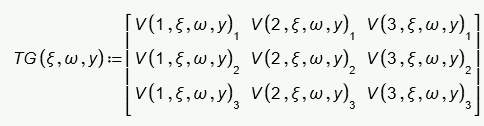
\includegraphics[width=0.5\linewidth]{Tgfor.png}
    \label{fig:enter-label}
    \caption{Green's tensor}
\end{figure}

The value (Figure 3.16) of Green's Tensor is:

\begin{figure}[h!]
    \centering
    
\includegraphics[width = 0.6\linewidth]{coupled_thermoelasticity/TG.PNG}
    \label{fig:TG}
    \caption{value of Green's tensor}
\end{figure}

To find solution of Green's Tensor need to get P matrix which is part of final formula defined as P matrix (Figure 3.17).

\newpage
\begin{figure}[htb!]
    \centering
    
\includegraphics[width = 0.6\linewidth]{coupled_thermoelasticity/P.PNG}
    \label{fig:P}
    \caption{define multiplication of arbitrary value and Green's tensor}
\end{figure}

The values of P matrix elements are around 1.0 (Figure 3.18):

\begin{figure}[htb!]
    \centering
    
\includegraphics[width = 0.6\linewidth]{coupled_thermoelasticity/Pres.PNG}
    \label{fig:Pres}
    \caption{Value of P matrix}
\end{figure}

The next part of formula is MM matrix (Figure 3.19).

\begin{figure}[htb!]
    \centering
    
\includegraphics[width = 0.6\linewidth]{coupled_thermoelasticity/MM.PNG}
    \label{fig:MM}
    \caption{Define multiplication of P and exp as MM }
\end{figure}

Finaly we need to find Green's Tensor.


\newpage
\section{IMPLEMENTATION IN MATLAB}
The temperature distribution over time, expressed as a function of temperature and position (Figure 4.1), depends on the specific system and the governing equations describing heat transfer within that system.

\begin{figure}[h!]
    \centering
    
\includegraphics[width=1\linewidth]{coupled_thermoelasticity/Graph.PNG}
    \caption{Temperature Distribution over time}
\end{figure}   


\subsection{Explanation of code}

In this section, we define the parameters (Figure 4.2) of the simulation. These parameters include the length of the rod (L), the total time for the simulation (T), the time step (dt), the spatial step (dx), and the thermal diffusivity (alpha).

\newpage
\begin{figure}[h!]
    \centering
    
\includegraphics[width=1\linewidth]{coupled_thermoelasticity/1st_sec.PNG}
    \caption{Parameters}
\end{figure}   

Here, we define the spatial grid (x) using the spatial step (dx) and the length of the rod (L). The Nx variable stores the number of spatial grid points (Figure 4.3).

\begin{figure}[h!]
    \centering
    
\includegraphics[width=1\linewidth]{coupled_thermoelasticity/2nd_sec.PNG}
    \caption{Spatial grid}
\end{figure}   



Similarly, we define the time grid (t) using the time step (dt) and the total simulation time (T). The Nt variable stores the number of time steps (Figure 4.4).

\begin{figure}[h!]
    \centering
    
\includegraphics[width=1\linewidth]{coupled_thermoelasticity/3rd_sec.PNG}
    \caption{Time grid}
\end{figure}   


We initialize the temperature matrix as a 2D array of zeros (Figure 4.5). This matrix will store the temperature distribution over both time and space.

\newpage
\begin{figure}[h!]
    \centering
    
\includegraphics[width=1\linewidth]{coupled_thermoelasticity/4th.PNG}
    \caption{Temperature matrix}
\end{figure}   


The initial temperature distribution along the rod at time t = 0 is set. In this example, it's defined as a sine function of spatial position (Figure 4.6).
\begin{figure}[h!]
    \centering
    
\includegraphics[width=1\linewidth]{coupled_thermoelasticity/5th.PNG}
    \caption{Initial conditions}
\end{figure}   


We set the boundary conditions. In this case, the temperature at both ends of the rod is kept fixed at zero (Figure 4.7).
\begin{figure}[h!]
    \centering
    
\includegraphics[width=1\linewidth]{coupled_thermoelasticity/6th.PNG}
    \caption{Set boundary condition}
\end{figure}   


We apply the initial temperature distribution to the first row of the temperature matrix (Figure 4.8).
\begin{figure}[h!]
    \centering
    
\includegraphics[width=1\linewidth]{coupled_thermoelasticity/7th.PNG}
    \caption{Initial condition}
\end{figure}   


The boundary conditions are applied to the temperature matrix (Figure 4.9). The first and last columns of the matrix are set to the values defined in boundary temperature.

\begin{figure}[h!]
    \centering
    
\includegraphics[width=1\linewidth]{coupled_thermoelasticity/8th.PNG}
    \caption{Set boundary temperature}
\end{figure}   


This section(in example Figure 4.10) implements the finite difference method to update the temperature distribution over time and space. It iterates over each time step (n) and each spatial grid point (i) and updates the temperature according to the discretized heat equation.

\begin{figure}[h!]
    \centering
    
\includegraphics[width=1\linewidth]{coupled_thermoelasticity/9th.PNG}
    \caption{finite difference method}
\end{figure}


Finally, the code plots the temperature distribution over time (Figure 4.11). It plots the temperature profile at every 10th time step for visualization purposes. The x-axis represents the spatial position, the y-axis represents the temperature, and each line represents the temperature distribution at a different time step.
\begin{figure}[h!]
    \centering
    
\includegraphics[width=1\linewidth]{coupled_thermoelasticity/10th.PNG}
    \caption{Display plot}
\end{figure}   


\bigskip


\newpage
\section*{\hspace{-1,25cm} \centering CONCLUSION}
\addcontentsline{toc}{section}{\textmd{CONCLUSION}}
\pagestyle{plain}
\indent

Formulas (2.93) allow us to model the dynamics of a thermoelastic
half-space for different boundary conditions: different sets of boundary
functions: displacements components, stresses components, temperature,
heat flow. Hence, presented approach allows us to solve different Boundary Value Problems
of coupled thermoelasticity if only 3 out of 6 of boundary functions are
known. On dependence of Boundary Value Problem, only the form of the matrix of the
resolving equations on the boundary \emph{S} must be changed.

The developed approach also provides a method for solving non-stationary
Boundary Value Problems for a thermoelastic half-plane. In this case, the solution (2.93) is
Fourier transform in time with non-stationary forces at the boundary and
zero initial conditions in the half-space. By performing inverse Fourier
transform in time of constructed solution, we shall receive the solution
of non-stationary problem. It is essential to require the possibility of
Fourier transforms of boundary functions.

This method allows to investigate the thermal stress-strain state of a
massif under the action of natural / artificial sources of thermoelastic
waves, acting on the surface and inside the massif. For internal
sources, the Cauchy problem for a thermoelastic space using the Green's
tensor of the equations of coupled thermoelasticity is solved first
{[}10{]}. Then the solution of the problem is determined as the sum of
received solution of Cauchy task by using this method.

This approach must find engineering applications in the problems of
geophysics and earthquake-resistant construction in the design of
surface and underground structures.

\newpage
\renewcommand{\refname}{\centering REFERENCES}
\bibliographystyle{unsrt}
\bibliography{references}
\addcontentsline{toc}{section}{REFERENCES}

\newpage
\section*{\hspace{-1,25cm}\centering APPENDIX}
\addcontentsline{toc}{section}{\textmd{APPENDIX}}

\begin{figure}[h!]
    \centering
    
\includegraphics[width=1\linewidth]{coupled_thermoelasticity/1app.PNG}
\end{figure}  

\begin{figure}[h!]
    \centering
    
\includegraphics[width=1\linewidth]{coupled_thermoelasticity/2app.PNG}
\end{figure}  

\begin{figure}[h!]
    \centering
    
\includegraphics[width=1\linewidth]{coupled_thermoelasticity/3app.PNG}
\end{figure}  

\begin{figure}[h!]
    \centering
    
\includegraphics[width=1\linewidth]{coupled_thermoelasticity/4app.PNG}
\end{figure}  

\begin{figure}[h!]
    \centering
    
\includegraphics[width=1\linewidth]{coupled_thermoelasticity/5app.PNG}
\end{figure}  

\begin{figure}[h!]
    \centering
    
\includegraphics[width=1\linewidth]{coupled_thermoelasticity/6app.PNG}
\end{figure}  

\begin{figure}[h!]
    \centering
    
\includegraphics[width=1\linewidth]{coupled_thermoelasticity/7app.PNG}
\end{figure}  

\begin{figure}[h!]
    \centering
    
\includegraphics[width=1\linewidth]{coupled_thermoelasticity/8app.PNG}
\end{figure}  

\begin{figure}[h!]
    \centering
    
\includegraphics[width=1\linewidth]{coupled_thermoelasticity/9app.PNG}
\end{figure}  

\begin{figure}[h!]
    \centering
    
\includegraphics[width=1\linewidth]{coupled_thermoelasticity/10app.PNG}
\end{figure}  

\begin{figure}[h!]
    \centering
    
\includegraphics[width=1\linewidth]{coupled_thermoelasticity/11app.PNG}
\end{figure}  

\begin{figure}[h!]
    \centering
    
\includegraphics[width=1\linewidth]{coupled_thermoelasticity/12app.PNG}
\end{figure}  

\begin{figure}[h!]
    \centering
    
\includegraphics[width=1\linewidth]{coupled_thermoelasticity/13app.PNG}
\end{figure}  

\begin{figure}[h!]
    \centering
    
\includegraphics[width=1\linewidth]{coupled_thermoelasticity/14app.PNG}
\end{figure}  

\begin{figure}[h!]
    \centering
    
\includegraphics[width=0.9\linewidth]{coupled_thermoelasticity/matlab1.PNG}
\end{figure}   

\begin{figure}[h!]
    \centering
    
\includegraphics[width=0.9\linewidth]{coupled_thermoelasticity/matlab2.PNG}
\end{figure}   

\end{justifying}
\end{document}